\documentclass{article}

% Load basic packages
\usepackage{balance}  % to better equalize the last page
\usepackage{txfonts}
\usepackage{times}    % comment if you want LaTeX's default font
\usepackage{color}
\usepackage{textcomp}
\usepackage{booktabs}
\usepackage{todonotes}
\usepackage{float}
\usepackage{url}  
\usepackage{titling}	% allows you to move title up the page
\usepackage[
  pdftex,
  pdfborder={0 0 0},
  linkcolor=red
]{hyperref}
\usepackage{xcolor} 
\usepackage{multicol}
\usepackage[margin=1in]{geometry}
\usepackage{graphicx}
\usepackage{capt-of}

% for code blocks
\usepackage{listings}
\usepackage{listings-golang} % import this package after listings

\definecolor{dkgreen}{rgb}{0,0.6,0}
\definecolor{gray}{rgb}{0.5,0.5,0.5}
\definecolor{mauve}{rgb}{0.58,0,0.82}

\usepackage{color}
\definecolor{lightgray}{rgb}{.9,.9,.9}
% \definecolor{darkgray}{rgb}{.4,.4,.4}
% \definecolor{purple}{rgb}{0.65, 0.12, 0.82}


\lstdefinelanguage{Dart}{
  keywords={var, String, int, List},
  ndkeywords={findAllElements,findElements},
  morecomment=[l]{//},
  morecomment=[s]{/*}{*/},
  morestring=[b]',
  morestring=[b]",
  keywordstyle=\color{blue}\bfseries,
  ndkeywordstyle=\color{purple}\bfseries,
  identifierstyle=\color{black},
  commentstyle=\color{purple}\ttfamily,
  stringstyle=\color{red}\ttfamily,
  sensitive=true
}

\lstdefinelanguage{TypeScript}{
  keywords={undefined, boolean, number, string, break, case, catch, continue, debugger, default, delete, do, else, false, finally, for, function, if, in, instanceof, new, null, return, switch, this, throw, true, try, typeof, var, void, while, with},
  morecomment=[l]{//},
  morecomment=[s]{/*}{*/},
  morestring=[b]',
  morestring=[b]",
  ndkeywords={class, enum, interface, export, boolean, throw, implements, import, this},
  keywordstyle=\color{blue}\bfseries,
  ndkeywordstyle=\color{purple}\bfseries,
  identifierstyle=\color{black},
  commentstyle=\color{purple}\ttfamily,
  stringstyle=\color{red}\ttfamily,
  sensitive=true
}

\lstset{
   language=TypeScript,
   backgroundcolor=\color{lightgray},
   extendedchars=true,
   basicstyle=\footnotesize\ttfamily,
   showstringspaces=false,
   showspaces=false,
   numbers=left,
   numberstyle=\footnotesize,
   numbersep=9pt,
   tabsize=2,
   breaklines=true,
   showtabs=false,
   captionpos=b
}
\renewcommand{\lstlistingname}{Code Snipped}
%%%%%%%%%

% Foot note line size
\renewcommand{\footnoterule}{%
  \kern -3pt
  \hrule width \textwidth height 0.5pt
  \kern 2pt
}

% font  sizes
\usepackage{sectsty}			% set font sizes			
\sectionfont{\Large}			% (assumes default font size 10pt)
\subsectionfont{\large}
% \subsubsectionfont{\large}
\subsubsectionfont{\normalsize}
\paragraphfont{\normalsize}

% positioning
\setlength{\parindent}{0em}		% remove indent for new paragraph
\setlength{\parskip}{1em}		% space above paragraph
\setlength{\columnsep}{2em}		% distance between columns
\setlength{\droptitle}{-10em}

% llt: Define a global style for URLs, rather that the default one
\makeatletter
\def\url@leostyle{
  \@ifundefined{selectfont}{\def\UrlFont{\sf}}{\def\UrlFont{\small\bf\ttfamily}}}
\makeatother
\urlstyle{leo}

% This is a constant to space out the section titles from their body
\newcommand{\vspaceconst}{-2ex}

% For notes
\newcommand{\TODO}{\textbf{\textit{\textcolor{red}{TODO:}}} }
\newcommand{\NOTE}{\textbf{\textit{\textcolor{red}{NOTE:}}} }

% For my sanity
\newcommand{\tpt}{\textit{`tracking point type'}}
\newcommand{\tpts}{\textit{`tracking point types'}}
\newcommand{\tp}{\textit{`tracking point'}}
\newcommand{\tps}{\textit{`tracking points'}}
\newcommand{\tg}{\textit{`tracking group'}}
\newcommand{\tgs}{\textit{`tracking groups'}}

% Setting the ToC depth level
\setcounter{tocdepth}{2}

\title{Honours Project Report\\Fitness Logger with Micro-services}
\author{Dumitru Vulpe\\BSc (Hons) Applied Computing\\Supervised by Andrew Colby}
\date{May 2021}

\begin{document}

\maketitle

\vspace*{\fill/2}
\begin{abstract} 

However, the main appeal of this project is the backend implementation. This is because as a part of the architecture design process, it was decided that a micro-services structure would be followed. Where the backend would be split up into multiple applications which would talk to each other where needed. This was chosen for a multitude of reasons, including as a learning experience for this kind of backend architecture.\\

\end{abstract}
\vspace*{\fill}

\newpage
\tableofcontents 
\listoffigures
\newpage

\begin{multicols}{2}
\section{Introduction}
\vspace{\vspaceconst}

This project is split into two main objectives; first objective was to to be a learning experience of creating a full stack application beginning to end and more importantly to get into micro services backend development. The second objective was to attempt to solve a problem which exists in the fitness industry by creating an application which would be useful to a different range of people and potentially taking this product to the market.\\

\subsection{Why micro services}
\vspace{\vspaceconst}

  The basic principle of micro services as opposed to a monolith, is to split up the backend application into multiple smaller applications. For example, in theory, a service such as Amazon (the online store), could have a separate micro service for the cart function, one for item listings, user account management, one for payment and more.\\
  Micro services architectures are becoming more and more relevant simply because the industry is getting becoming more and more complex. As size, complexity and number of users increase, so does the need for well scaled web applications. Micro services type architectures are simply one way to cleanly and easily scale web applications. So because of industry relevance and my personal enthusiasm, it was decided that this project's backend would also follow this architecture. See figure~\ref{fig:monoVsMicro} for a visual representation of this concept.\\

\begingroup
\centering
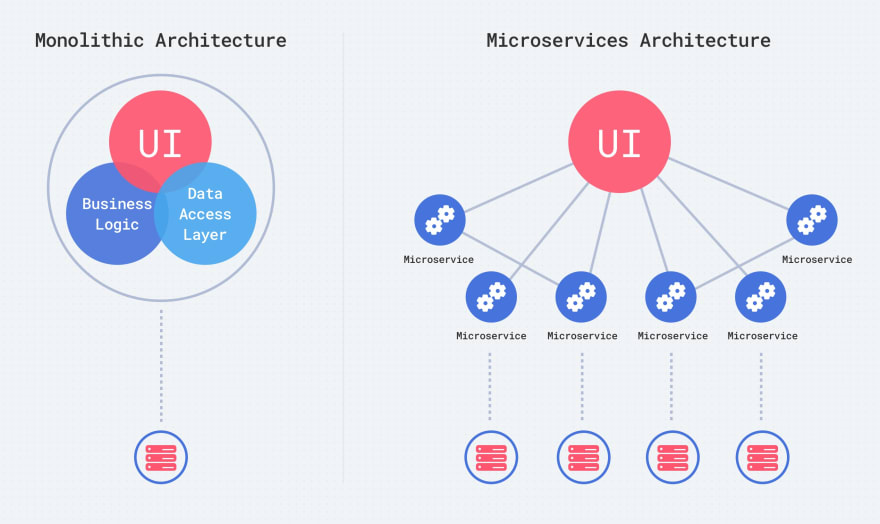
\includegraphics[width=0.9\linewidth]{./miscAssets/monoVsMicro.jpg}
\captionof{figure}{Monolithic vs micro services architectures}
~\label{fig:monoVsMicro}
\endgroup

\subsection{Creating a potential product}
\vspace{\vspaceconst}

Creating a fully fledged product out of this project was not the main intention. However, in in the author's personal opinion, the planned solution for the problem has enough potential that could work as a product in the market. And as long as the application works as intended, there are multiple potential monetisation routes which could be taken, such as extra features behind a subscription or just a flat rate at purchase.\\

\subsubsection{The problem}
\vspace{\vspaceconst}

From past experience, the author has not yet found a simple, fuss free, yet flexible application for logging workout sessions and related notes for said session. The applications which were tried so far are either made for specific workout programs or are not complete, buggy or just do not have enough flexibility in the type of logging one can achieve. It often feels like fighting an uphill battle when using one of these applications.\\
In the fitness world there can be a lot of different types of workouts, exercises, exercise variations, and ways to do said exercises. Because of this, coaches, personal trainers and everyday people usually would stick to using a notepad and pen simply because there are no arbitrary restrains on what you can log, either that or or not log the workouts in general.\\
Typically a notepad and pen is not a bad solution and usually preferable to most applications, however, there are certain drawbacks to this approach. One practical drawback is highlighted when working out in a commercial gym, walking around the gym using different equipment and carrying everything one might need including the notebook and pen combo can be quite cumbersome, same goes for actually noting down the data in the notebook. When it comes to looking back on previous workouts it can also be quite cumbersome, especially when you are in the middle of a workout and do not want to loose the tempo. And the other reason being that compiling analytical data from a notebook can be tedious and take time. Computers are much better at calculations and statistics.\\

\subsubsection{My planned solution}
\vspace{\vspaceconst}

The idea was that the system would be designed around the data structures needed, one of which would be chosen by the user. This data structure would be made as simple as possible while still allowing all the common basic exercise options (such as repetitions, resistance values, sets etc) but also others (such as the option to just write a single value). Furthermore, the system would allow the user to create their own exercise types which they would then use when logging a workout.\\
When using the application the user would first create a custom `type'. This type would usually be an exercise, however, it it not constrained to be one. For example, one type would be `exercise x' and another type could be `caffeine intake' for tracking the intake of caffeine over different workouts. Then, the user would able to create logs based on those custom types.\\

\section{Background}
\vspace{\vspaceconst}

\subsection{Architecture design}
\vspace{\vspaceconst}

A lot of time during this project was allocated to research of the backend architecture design, specifically relating to micro services. And when it comes to it, there is not just one or few generally accepted standards and patterns that projects adopt. This is simply because, from all of the articles and talks that exists online from system architect, each and every architect needs to answer a lot of questions about it will all be built.\\
 For instance, the questions about how the different services should be split, some say it should be split by the feature, some say by the individual data element, by endpoint and more. Another popular questions is how the services diagram should look like, one of the popular answers are to have a separate authentication service to provide authentication for the application and proxy the requests to all the other services. However, regardless of the question, there are a lot of different ways solutions to all of these questions that need to be answered when starting a project using micro services and all of them come with their own advantages and disadvantages.\\

\subsubsection{Helpful technologies}
\vspace{\vspaceconst}

  When creating micro service systems, there are a lot of technologies which could and would be used to make the development of these services easier. Probably one of the first pieces of technologies to ease the development and deployment of micro services a lot easier are containers. Containers allow you to package applications with all of the needed dependencies and environments, they virtualise the user-land applications\footnote{User-land application are all the program running on a computer that do not run on the same level as the kernel.} and share the host's kernel. On a Linux system, that means that containers can virtually run under any distribution\footnote{Distribution of Linux is referring to different operation systems built on the Kernel}.On non-Linux systems, these containers would usually be inside a Linux virtual machine. Furthermore, container management and orchestration solutions also exist, technologies such as Docker\cite{Docker}, docker-compose\cite{Docker} Docker Swarm\cite{Docker}, Kubernetes\cite{k8s} and more. These help with running the actual containers, and in the case of Kubernetes, it also allows us to easily define configurations and scale the containers either on a definition or on demand. Scaling here would be done by running more instances of that container across a cluster of machines running the Kubernetes and load balancing the traffic amongst them. This is known as horizontal scaling (see figure~\ref{fig:ScaleOutVsIn} for a comparison of horizontal vs vertical scaling).\\
  Micro services would often also need to talk to each other and as before, depending on requirements and design, there are different ways to do it. Overall, there are two options many systems using both synchronous and asynchronous calls. Synchronous calls are usually straight forward and done over HTTP and the only thing that would need to be solved is proper authentication. Asynchronous calls are often made with either RPC\footnote{RPC or Remote Procedure Calls is an inter process communication technique used to call subroutines between applications.} calls (commonly gRPC\cite{grpc} would be used) or a message/event bus system such as Kafka\cite{kafka}.\\
Another great series of helpful technologies are service meshes, they provide great insight into your cluster of micro services. It is a dedicated infrastructure layer that all the different micro services would proxy their communication in-between. This can provide a multitude of benefits including communication observability, call chain traceability, secure connections and more. Examples of such services are Linkerd\cite{linkerd} and Istio\cite{istio}. If this project would be using Kubernetes, a service mesh would definitely be very useful and worth wile to integrate into the system.\\

\subsection{Market}
\vspace{\vspaceconst}

One of the applications that the author had experience with was `Zero to Hero'\cite{zerotohero}. This is a workout application which mostly revolves around giving the users different workout programs to follow, it also calculates they weight they should be using based on the max weight the user can do. Then as the workout is performed, the user can log it. However, the problem with this application is its complexity and bugs. The complexity it has stems from the workflow the user would go through. An user cannot simply just open the app and start logging, first the user needs to chose from a program, then the user needs to follow the program precisely. And on top of that a user cannot make their own workouts or exercises. A majority of the workout logging apps tend to function in this manner.\\
So, to reiterate, there are a fair amount of apps which cater to the fitness market, however, there seems to be a small gap in the market where there aren't many options for a workout logging app which does just logging of one's own custom experiences.\\

\section{Specification}
\vspace{\vspaceconst}

\subsection{Micro services}
\vspace{\vspaceconst}

The proposed project is tackling two main problems, one being a whole set conceptual problem which are very common with increased project sizes, weather that is in terms of complexity, code base, team size or general scope of the project. So it is generally welcome to try and apprehend for these problems ahead of time by careful planning and designing of the system. In this case, the careful planning and designing would be done on the backend architecture. Here, using micro services would solve a lot of problems, both technical and business problems.\\

\subsubsection{Business \& general project management problems}
\vspace{\vspaceconst}

When a project grows in size to the point where there is a need for multiple teams it can become quite challenging to have all of the teams work on the same code base. Different tactics such as smart management of the version management system could help with this issue. One such example would be to have different development branches for each team, however, this could introduce more problems such as needing to re-base the branch mid development. Here, a much better way would be to simply have the teams work on different codebases, each making up a micro service. Depending on how the teams are organised, or on how the features are broken down in each micro service, each team would be solely responsible of one or more micro services, making them the de facto experts on that specific micro a service and its inner workings.\\
What about when new individuals or teams enter the workforce? There is usually a fair amount of time taken just simply getting acclimated with the codebase and the whole product. Now, this would be true weather the project is or is not following a micro services architecture, however, if the project is just a monolith, usually the individual or team would need to get familiar with the while codebase. This would not need to be true in case of micro services.\\
With micro services the individual or team would just need to look at the API documentation of the project, then only get accustomed with the micro service that they would be working on. This way collaboration between teams also will become easier due to each team maintaining their own small codebases and API documentation, making it easier to consume the API.\\

\subsubsection{The technical aspect}
\vspace{\vspaceconst}

Originally projects would just be one monolithic application and if we needed more performance we would optimise the code and add more power through better server hardware (or add more resources to the virtual machine or container if it was applicable). This is called vertical scaling. However, what happens when we need even more scaling? There can only be so much power we can add to one single server and only so much optimisation we can do to a codebase. Projects then started to scale their applications horizontally by deploying more instances of it, then adding some form of a load balancer which would balance the requests across all of their different deployments. These deployments could be individual computers, running the application directly on bare metal\footnote{Bare metal meaning that there is no other layer of management such as virtualisation or containerization and is running directly on the host OS.}. This, however, could be quite inefficient because it would scale the whole application and this might not be needed but also because applications typically would not be able to utilise 100\% of the resources the system has to offer.\\
For example, assume \textit{Application x} has a user profile endpoint which is just a simple CRUD\footnote{Referring to data operations of Create Read Update Delete.} operation and a pictures endpoint which is responsible for handling picture uploads, picture compression, storage, serving, etc. The part which will need the most processing power will be the pictures endpoint, but when vertically scaling a monolith, all of the endpoints get deployed again regardless if they needed the extra resources or not. This in principle is wasted resources and by extension wasted budget for a project.\\

\begingroup
\centering
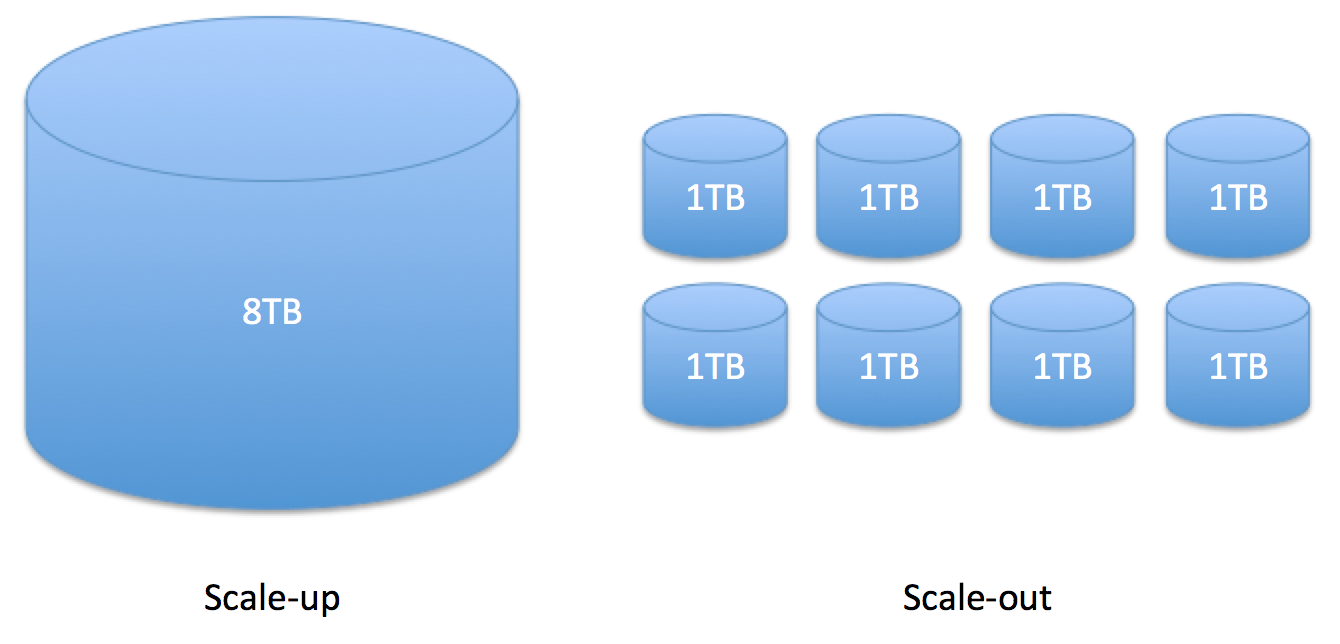
\includegraphics[width=0.9\linewidth]{./miscAssets/ScaleUpVsScaleOut.png}
\captionof{figure}{Scaling out vs scaling in}
~\label{fig:ScaleOutVsIn}
\endgroup

Note figure~\ref{fig:ScaleOutVsIn}, this is an example of vertical scaling (or scaling up) versus horizontal scaling (scaling out) for a file system. \\

\subsubsection{Solution}
\vspace{\vspaceconst}
As it turns out, micro services architecture, plus technologies such as Docker and Kubernetes solve this exact problem by having each feature/endpoint/verb/structure on a different service then vertically scaling each service when needed with a load balancer re-directing the traffic to instances.\\
In the long term this will also save on resources because developers will not need to spend as much time on writing code which can will take complete advantage of all of the computing resources available to it.\\

\subsection{The application}
\vspace{\vspaceconst}

When it comes to logging any sort of fitness activities, there is no standard, and there are a lot of different ways an individual or a trainer might log these activities; there simply does not exist a \textit{one size fits all} solution or a generally accepted template to this. It all just depends on the goals of said person or trainer. Because of this it is gets fairly complex when it comes to trying to make a digital form which could be filled out and be able to process and display all the data from it in any meaningful way. Usually different applications would create a rigid structure for the data then there would be forms to input the data in. For some people that would work perfectly, but not for all especially across athletes from different disciples of sport.\\

\begingroup
\centering
\begin{tabular}{l l p{3cm}}
  \toprule
  \# & Exercise & Sets \\ [0.5ex]
  \midrule
  1 & Squat & 10x40kg, 10x60kg, 8x70kg, 8x80kg\\
  \midrule
  2 & Dead lift & 12x50kg, 12x70kg, 10x80kg, 8x100kg\\
  \midrule
  3 & Hack squat & 15x50kg, 15x60kg, 15x70kg, 12x70kg\\
  \midrule
  4 & Leg press & 15x40kg, 15x60kg, 15x70kg, 15x80kg\\
  \midrule
  5 & Ham string curl & 15x26kg, 15x32kg, 15x36kg, 15x32kg\\
  \bottomrule
\end{tabular}
\captionof{table}{Simple workout log example}
~\label{table:WorkoutLogExample1}
\endgroup

For instance, one of the simplest logging types would be just performing straight sets of different exercises, some exercises being done with weights, or some other form of resistance which would also be noted down with every set. Table~\ref{table:WorkoutLogExample1} shows one such example. However, as mentioned just now, it is a very simple form of logging and there are a lot more details that could be added, or a lot more variations that people could be doing which would need to be noted. Some examples are the following: \textit{super-setting}\footnote{Super-setting is performing a set of one exercise and another set of another exercise straight away without resting, then repeating the cycle.} and \textit{drop-setting}\footnote{Drop-setting is when the athlete performs another set without set at a smaller resistance, usually -20\%}. These are just some of the more common ones. However, not everyone will use these exercise techniques so not everyone will need to be able to log them. All of this adds extra complexity, which means an application for logging will either be very complex, or only useful to a subgroup of people with a specific workout style.\\

\subsubsection{Solution}
\vspace{\vspaceconst}
 
The premise to the solution in this project is quite simple, \textit{`keep it simple stupid'}. The solution which is being proposed it to simplify the data structure as much as possible while still including some of the minimum features such as drop-sets, super-sets, notes, measurement units, etc. But also let the user create their own custom exercises which they will keep track of, reuse and then be able to look back on their history. As an extension to this system, the actual exercise data (as opposed to the meta-data that has just been discussed, such as data about each set, see table \ref{table:WorkoutLogExample1}, sets columns for an example) is variable in type as well. At the moment there are only two sub-types implemented, a usual \textit{set} type and a \textit{single value} type which just logs one single value per exercise. This lets users be able to better track things such as static holds\footnote{Static holds are experiences where you hold a position for a duration of time.}.\\
An example use case would be people which would like to keep track of their caffeine intake for every single workout. So there would be a custom exercise type with the measurement unit of \textit{mg} made by the user which would be called  `Caffeine' and would have a data type of \textit{single value}. Then on each workout that the user starts, they would have the option to log a point of exercise type `Caffeine' with the amount of caffeine ingested.\\
There was also an initial intention to create a really flexible report/charting analytical system for all of the data stored by the user. That system would be using tags as its base concept, and everything would be `tagable'. Then based on those tags, the user would be able to perform searches and compiling reports and cross referencing data on charts.\\
For example, a user would be able to tag a workout as a \textit{de-load workout}\footnote{A de-load workout is when the athlete uses lower weights as a form of rest but still workouts.} with a \textit{`\#de-load'} tag. Then, the user would want to generate a report or a chart which would show all of the workouts but miss out the ones where he de-loaded by creating a filter for not including this tag.\\
These tags could also be used as a way to define the different workout splits\footnote{A workout split meaning the different muscle groups the workout is targeting, e.g. \textit{Chest and back day}.} such as \textit{`\#chest'} and \textit{`\#back'} for a chest and back workout.\\
This concept could even be done on a finer scale on a per-exercise type basis. Give each exercise tags for each muscle or muscle groups they are working out, then be able to look up the exercise base on those tags.\\

\subsection{Methodology}
\vspace{\vspaceconst}

This project was mostly split into three main parts, the research phase, the setup phase, and the development phase. The research phase being especially important because the author had no prior experience with such architectures and a lot of information had to be learned from scratch. For this reason, the requirements for the project had to be fairly flexible because there was uncertainly about what could achieved and what had to be left on the conceptual table.\\
The setup phase was about setting up the git repositories, an NPM library which was used as the shared code library amongst the projects, and a template which can be used for easier creation of extra services. Then, the last phase was actually split into multiple parts, the backend, the frontend and the testin//debugging phase.\\

\subsubsection{Milestones}
\vspace{\vspaceconst}
\begingroup
\centering
\begin{tabular}{l p{3.4cm} p{3.1cm}}
  \# & Milestone & Deadline\\
  \midrule
  1 & Research & Mid October to end of November\\
  2 & Setup & December\\
  3 & Backend development & January and February\\
  4 & Frontend development & March\\
  5 & Testing and troubleshooting & April\\
\end{tabular}
\captionof{table}{Mile Stone List}
\endgroup

For the most part, the schedules milestones which were set has been followed, only slightly deviating at the end and taking one week longer with the frontend development due to inexperience with the UI framework being used.\\
To split this down further, there were some mini milestones set for each micro service, of which there were 3: \textit{`fl-auth'}, \textit{`fl-tp-types'} and \textit{`fl-tp'}. With \textit{`fl-auth'} taking two weeks to complete, and the other two micro services taking 3 weeks each. Although, this is without any proper integration testing and troubleshooting. Some of that had to be done while building the frontend when consuming the API.\\

\subsubsection{Project management}
\vspace{\vspaceconst}

Since this project is developed by a single developer, there was not much need for standalone project management tools such as a GitHub Projects page or a Kanban board. From the author's past experiences these kind of tools are mostly useful when collaborating with other people on the same project, and when working on projects alone, it can actually become more work to just maintain and update such a system.\\
Since the beginning, there was a complete understanding of what the end goal of this project was, complete with a rough MVP\footnote{MVP stands for Minimal Viable Product} and stretch goals for the project. Therefore, there was no need to have that broken down into individual stories for a backlog. So for the majority of the development, the author only kept a to-do list in his personal journal. The only needing a Kanban board when bugs started uprearing, so that was basically a bug tracking system, but also for small improvements which were thought about on the spot. This came in the form of a physical Kanban board with post it notes for stories. There was one for the backend (refer to figure~\ref{fig:backendKanban}) and one for the frontend (refer to figure~\ref{fig:frontendKanban}).\\

\begingroup
\centering
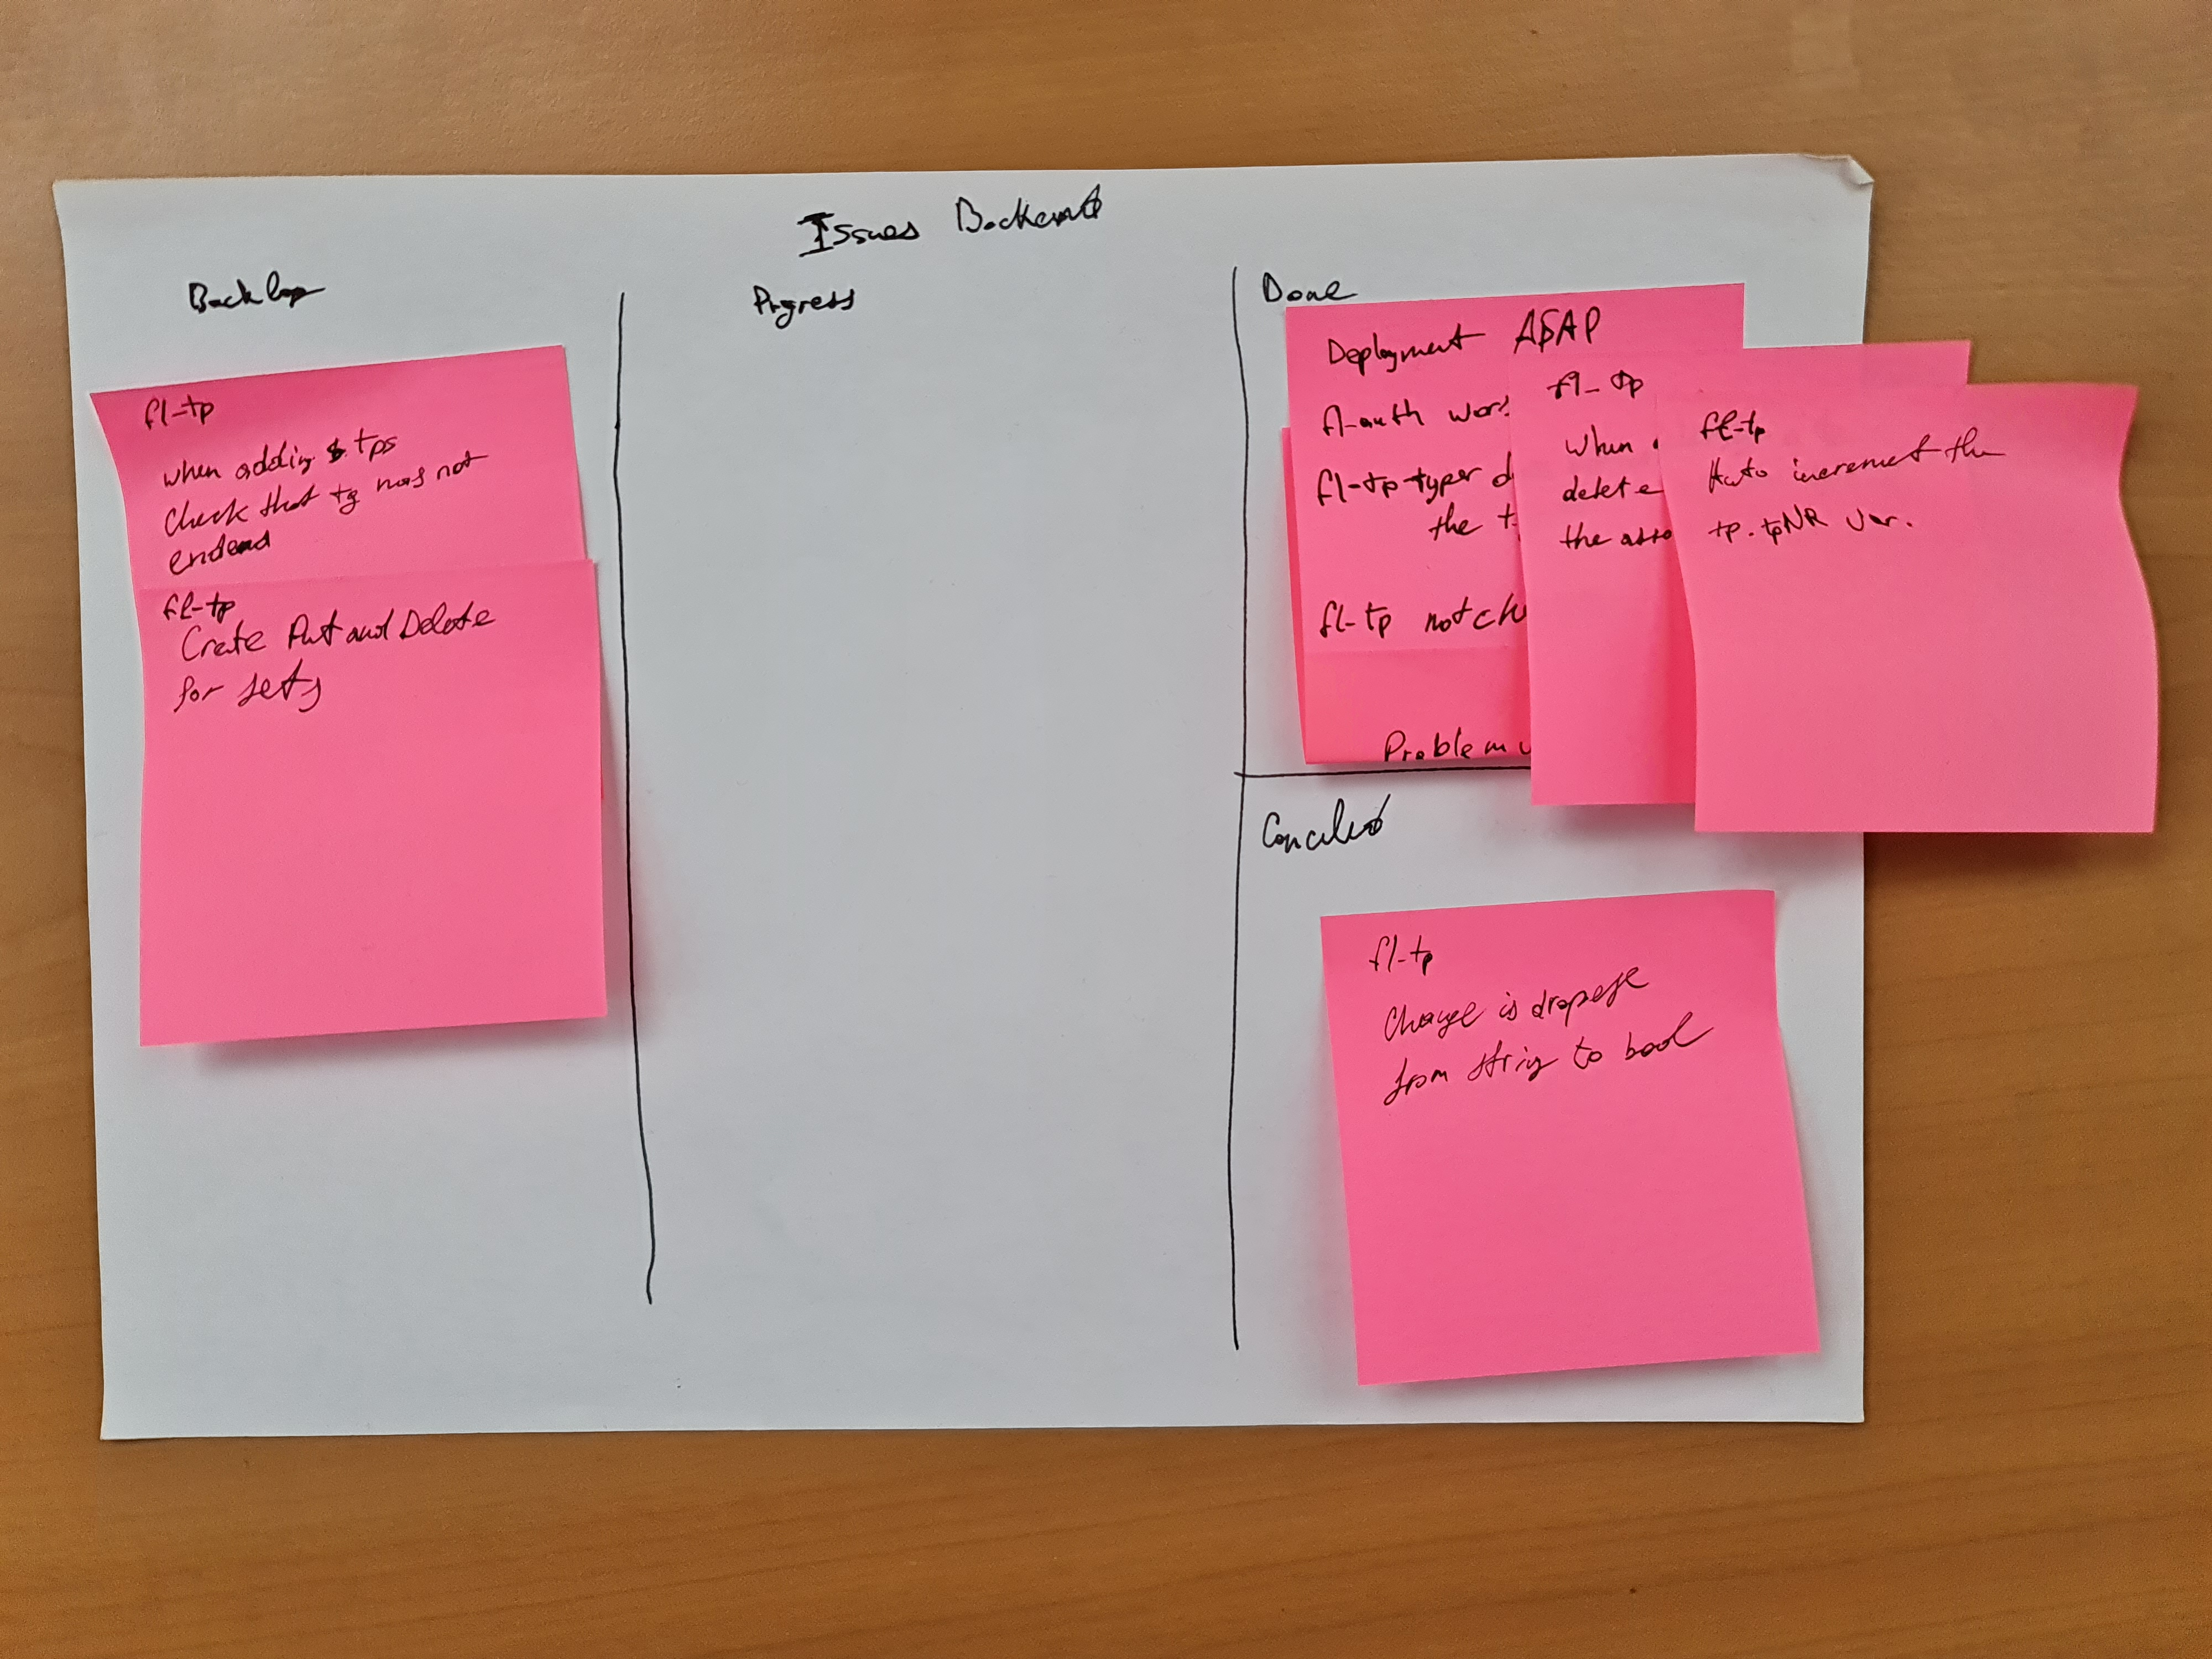
\includegraphics[width=0.9\linewidth]{./appendix/assets/img/backendBacklog.jpg}
\captionof{figure}{Backend Kanban Board}
~\label{fig:backendKanban}
\endgroup

\begingroup
\centering
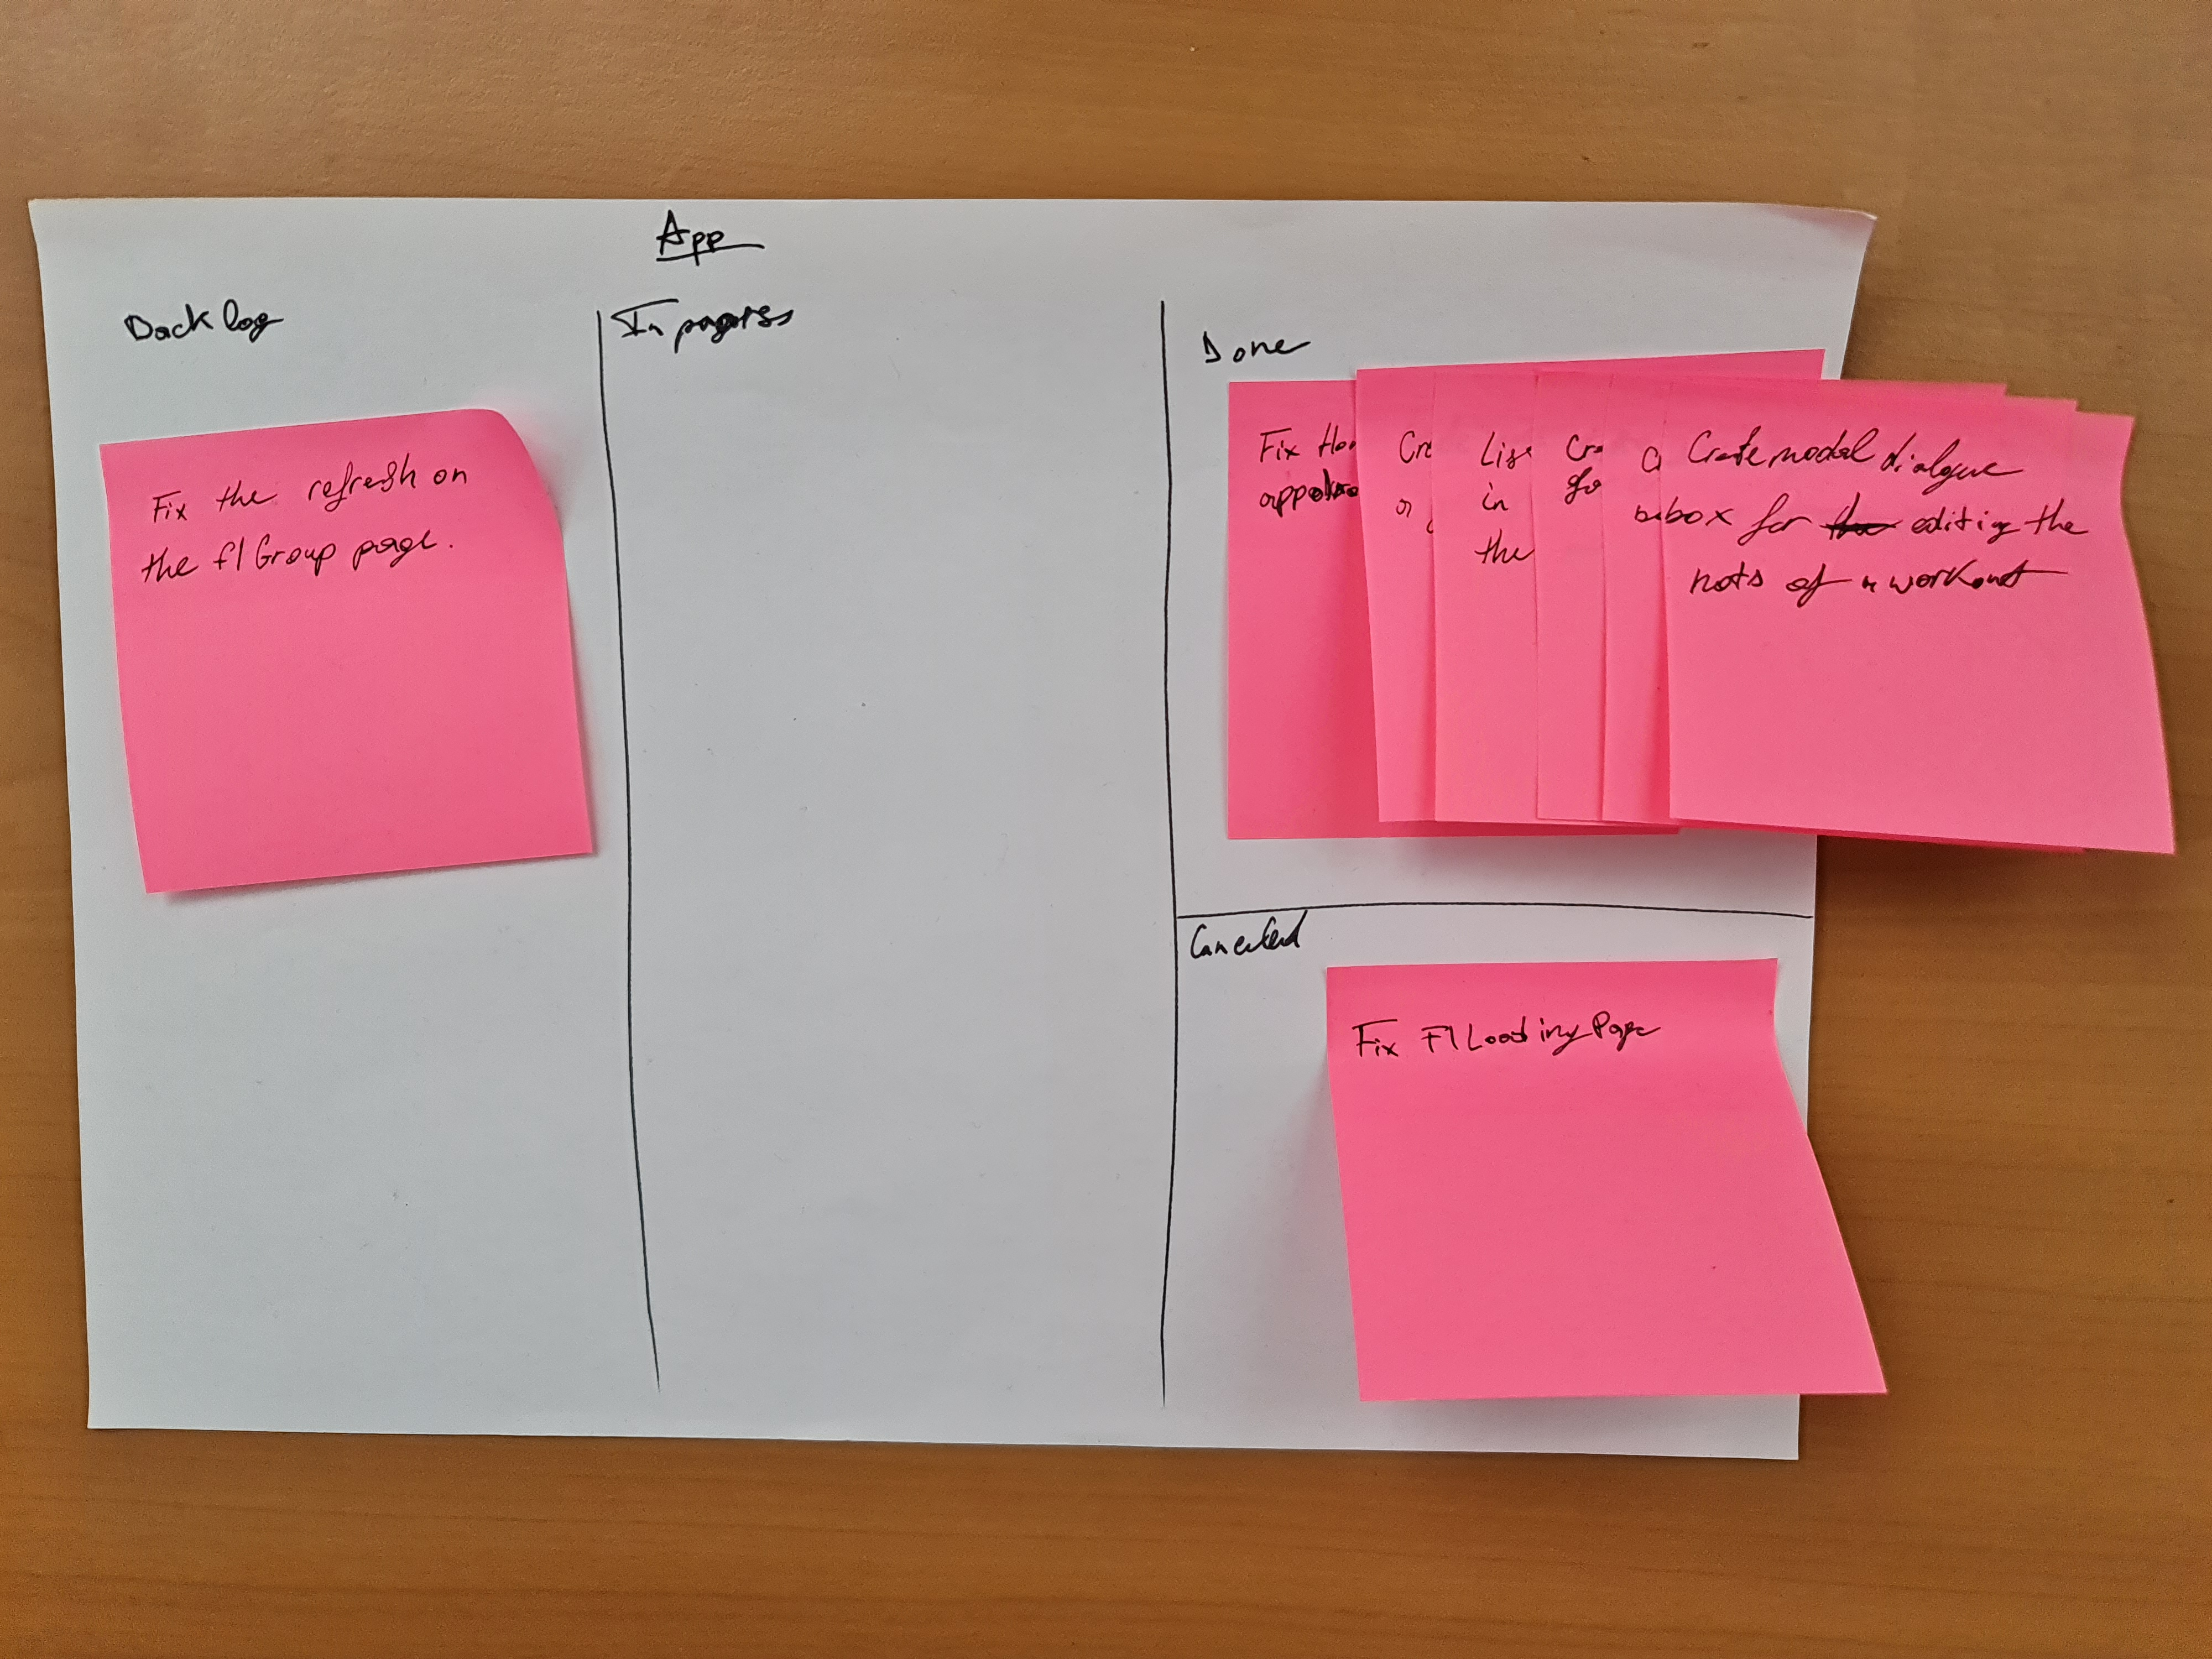
\includegraphics[width=0.9\linewidth]{./appendix/assets/img/frontendBacklog.jpg}
\captionof{figure}{Frontend Kanban Board}
~\label{fig:frontendKanban}
\endgroup

Even though it is thought that this project could be taken on the market with a seeming advantage other other apps, the main client for this application is the author himself. For this reason the wanted functionality of the project was known from the start, so then the requirements and deliverables were set in stone (example of draft one of requirements document in figure~\ref{fig:flReqDoc}). This means that there was no need for an iterative `Agile'\footnote{As written on Atlasian's page\cite{agile}: `Agile is an iterative approach to project management and software development that helps teams deliver value to their customers faster and with fewer headaches. Instead of betting everything on a \"big bang\" launch, an agile team delivers work in small, but consumable, increments. Requirements, plans, and results are evaluated continuously so teams have a natural mechanism for responding to change quickly.'} style approach to development. Meaning there was no need to agile sprint cycles.\\
The approach used here was one of an \textit{`adaptive waterfall'} method. Meaning that there was already a good idea what the final product would look like and only made small adjustments in the plan as it made sense during the development phase.\\

\begingroup
\centering
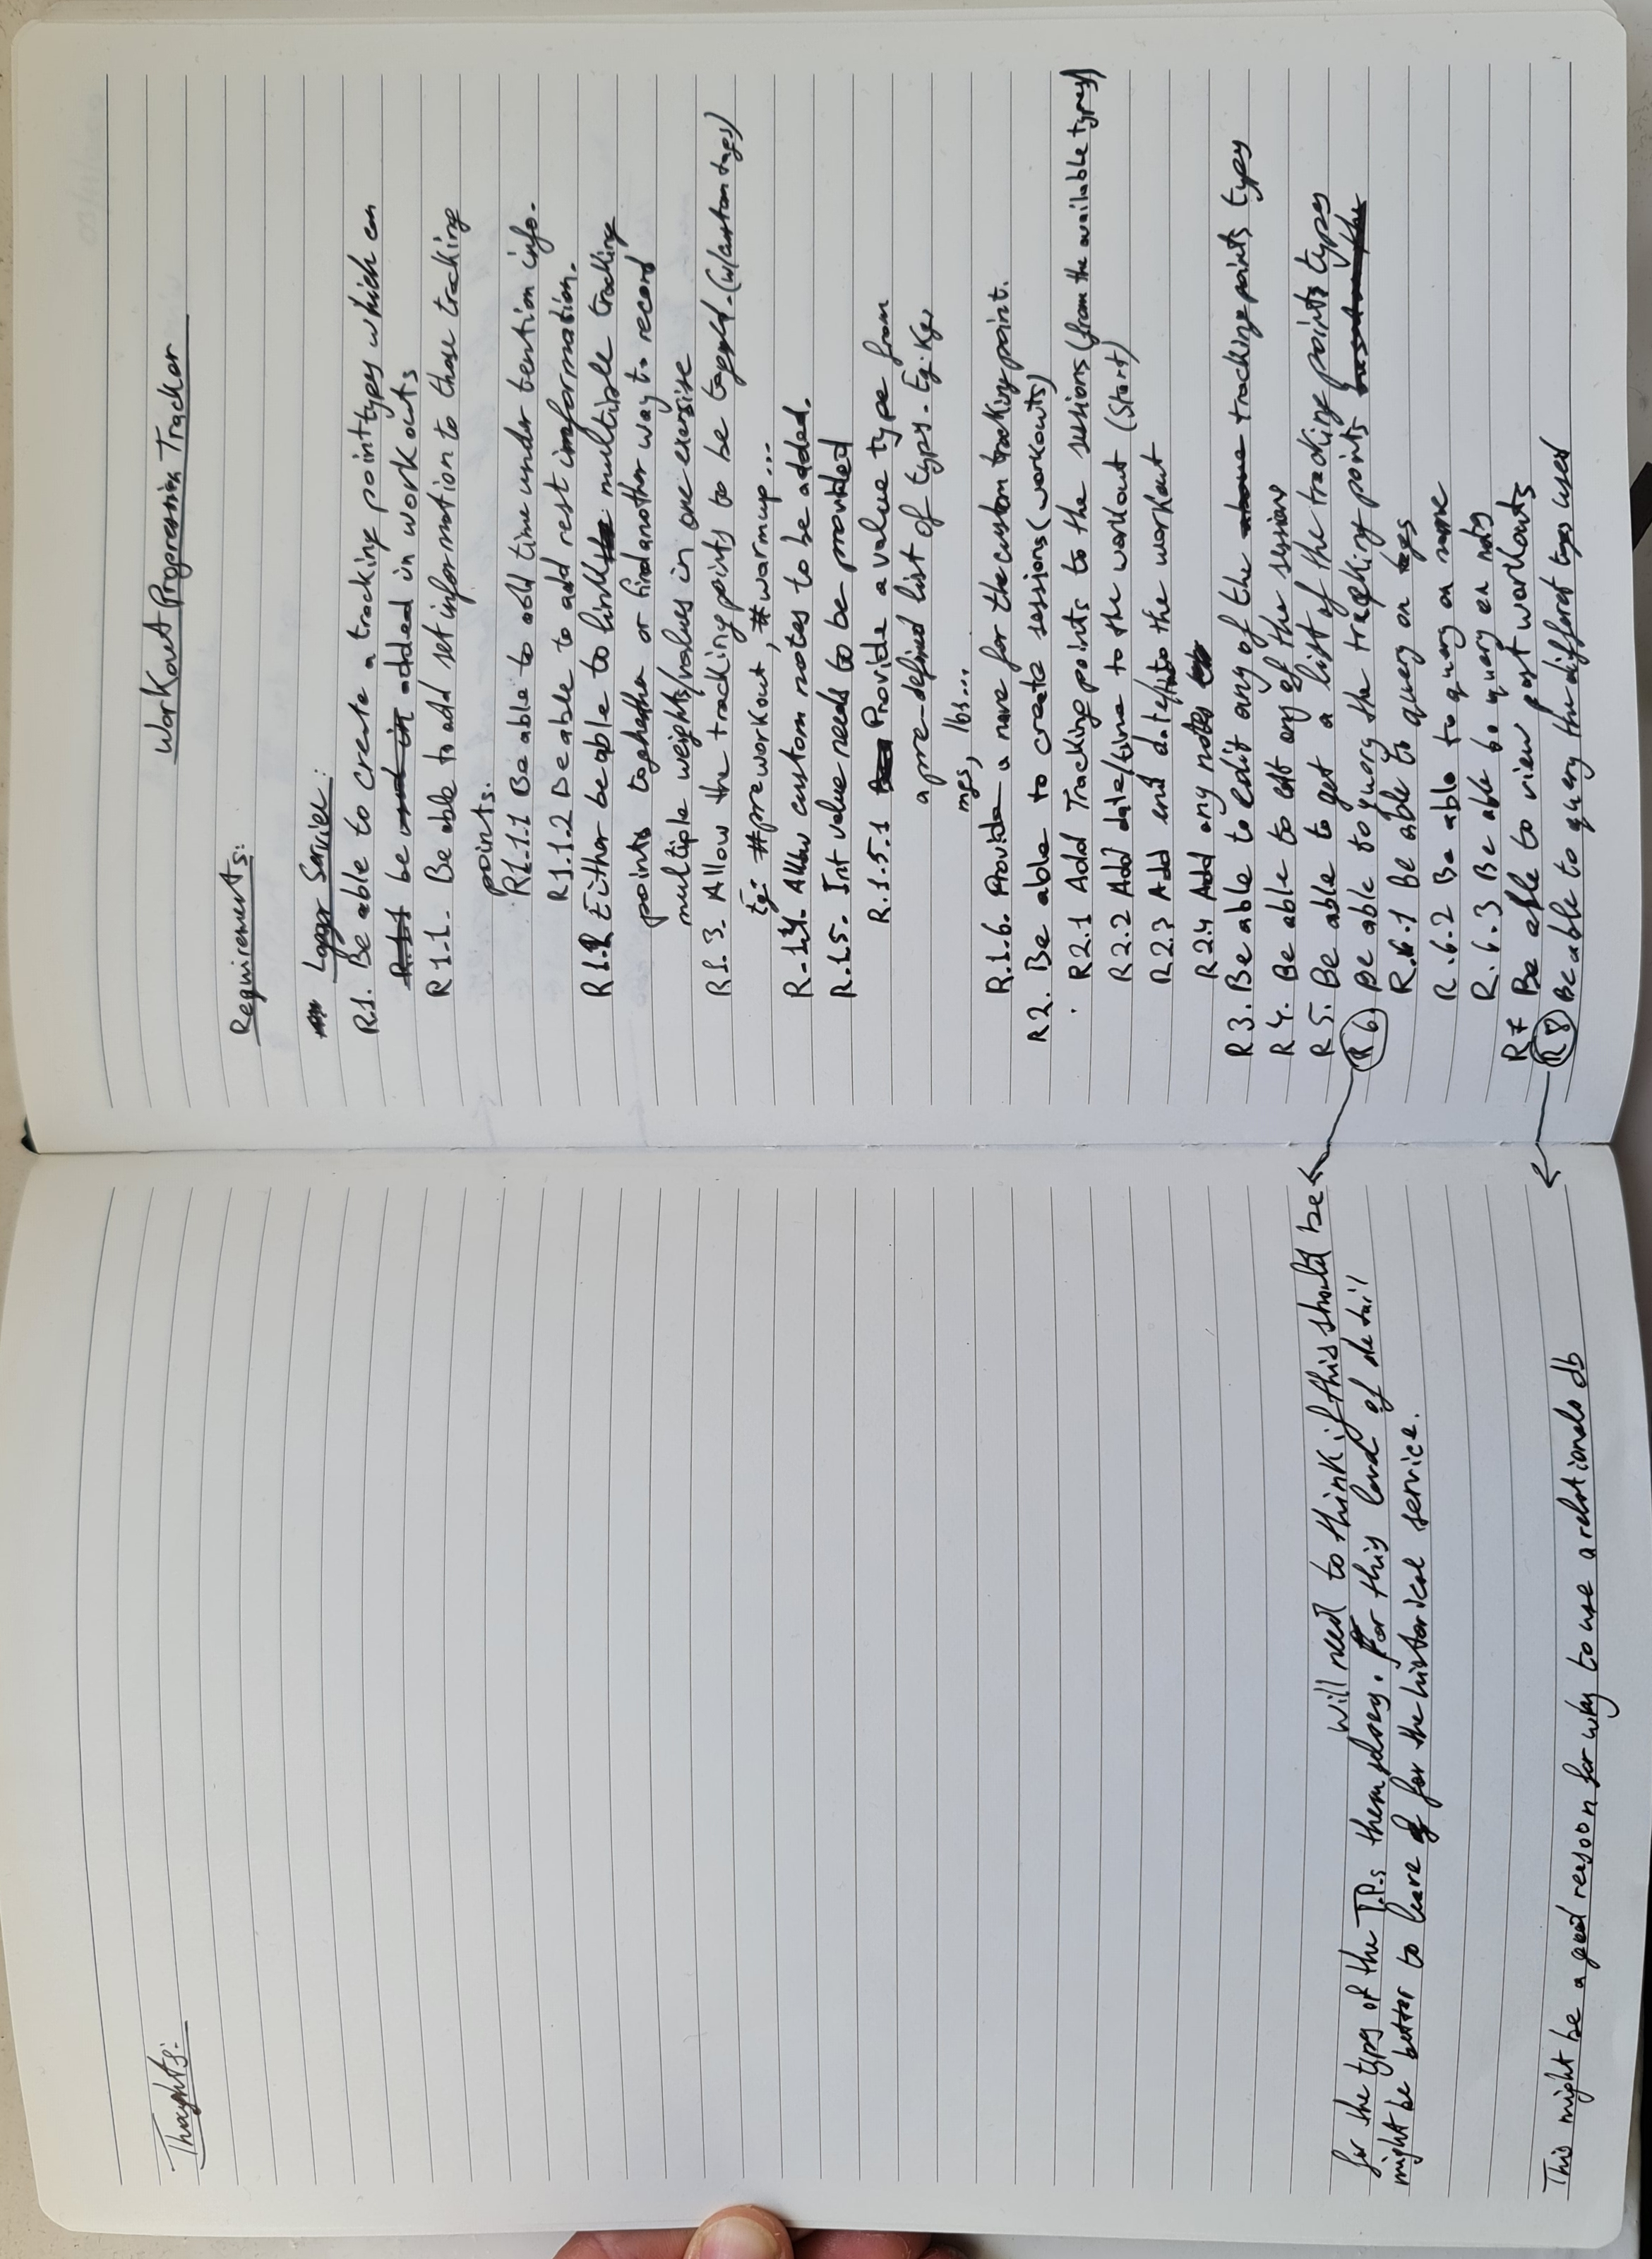
\includegraphics[angle=270,origin=c,width=0.9\linewidth]{./appendix/assets/img/initialRequirementDocument.jpg}
\captionof{figure}{Fitness Logger Initial Requirements Document}
~\label{fig:flReqDoc}
\endgroup

\section{Design}
\vspace{\vspaceconst}

\begingroup
\centering
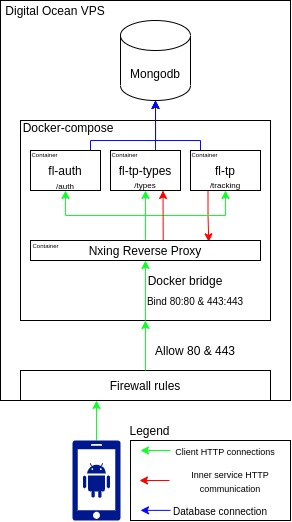
\includegraphics[width=0.7\linewidth]{./appendix/assets/charts/fitnessLogger.jpg}
\captionof{figure}{Fitness Logger Architecture}
~\label{fig:flChart}
\endgroup

Even though micro services usually can increases the hugely complexity, this project stayed relatively simple. Figure~\ref{fig:flChart} shows a general diagram for this project which is largely made up of 3 parts, the client application, the docker container running an Nginx reverse proxy forwarding the traffic to the services,the docker containers running the services and the database management system, MongoDB in this case.\\

\subsection{Technological design}
\vspace{\vspaceconst}

\subsubsection{Database}
\vspace{\vspaceconst}

The database management system that was chosen for this project was MongoDB.\@ This is a document object storage database (aka No SQL db), meaning it stores JSON\footnote{JSON stands for JavaScript Object Notation and it is a data formatting standard used for sending data over networks, saving data to files and more.} objects which can potentially have a tree like structure, which is actually important to some of the data which the project will be storing. Other than MongoDB being able to store object trees another reason why it was chosen was because of its ease of use with virtually any programming language. For example, in NodeJS, a read operation would be just as simple as \textit{'collection.findOne({})'}, just providing a JSON or a BSON\footnote{BSON stands for Binary JSON which is just binary encoded JSON model.} object with the search parameters matching the field names in the database. A create operations is even simpler, \textit{`collection.insertOne(data)'}, with data being any kind of JSON serializeable object.\\
The alternative DBMS system which was considered for this project was Posture SQL. This is probably the best SQL system from a point of view of features and speed. However, the more considered it was the more it was realised that there is no point of using a relational database because the relations would have to be defines on the backend application side. That is because, if the different services where to interact with each other's database, or were all to use the same database, it could potentially case problems with data integrity on the database side. So, it is generally accepted as good practice that all micro services would have their own database, and if they needed to read or write data to another micro service's database, they would do it through their API.\@ Also, MongoDB offered the project the flexibility to use nested JSON objects which ended up being used in the \textit{`fl-tp'} service (see section \ref{sec:dataStruct}).

\subsubsection{Data structures}\label{sec:dataStruct}
\vspace{\vspaceconst}

As mentioned before, one way to solve the problem of workout logging which was stated was to be create simple data structure which could be used in flexible ways in conjunction with their own custom \tpts by the users of the application.\\
So, the current data structure design is split into three parts, \tps, \tgs and \tpts. \textit{`Tracking point types'} is the first data structure to have been made, it contains information about each individual custom exercise, or any other tracking point the user might want to create. Code snippet~\ref{code:tptStruct} is the data structure used inside the \textit{`fl-tp-type'}, it allows the user to define their own measurement units, in case the experience uses some arbitrary resistance values; and last but not least we have the data type, this is an enum which tells \textit{`fl-tp'} micro service what kind of data this type will store. At the moment there are only two types of data, however, this could be expanded in the future, and theoretically could even add user definable data types.\\

\begin{lstlisting}[escapeinside={(*}{*)}, label={code:tptStruct},caption={Tracking Point Types Data Struct}]
export enum DataType {
    Sets = 'sets',
    SingleValue = 'single-value',
}

/* ITrackingPointTypes interface for typescript. */
export interface ITrackingPointTypes {
    userId: string;
    tpName: string;
    description: string;
    dataType: DataType;
    measurementUnit: string;
}
\end{lstlisting}

The next data structure is one of the simplest ones, it is used to store meta data about each \tg~(code snippet~\ref{code:tgStruct}). An example of a \tg~could be one workout which would have multiple \tps. So a \tg~would have meta data about start time, end time, and notes about the workout. The reason why there is no \tps~inside this typescript interface. Note, the variable definition on line~\ref{code:tgStruct:endTime} of Snipped~\ref{code:tgStruct} is of type \textit{`number $\vert$ undefined'} the reason for that is that when a \tg is first created it will not have an end time, so at first it is set to null.\\

\begin{lstlisting}[escapeinside={(*}{*)},label={code:tgStruct} ,caption={Tracking Group Struct}]
export interface TrackingGroup {
    userId: string;
    startTime: number;
    endTime: number | undefined; (*\label{code:tgStruct:endTime}*)
    notes: string;
}
\end{lstlisting}

The \tp data structure (code snipped \ref{code:tpStruct}) is the most important one, this is the actual structure for the exercise data or as it is referred to internally, \tps. It holds some meta data about the exercise but also the data of the exercise itself which, the type of that is retrieved from its corresponding \tg. This is part of what makes this system so flexible. A user is able to create their own type of workout, with potentially limitless types of data, then be able to log that kind of type of data into the database. Line \ref{code:tpStruct:dataTypes} of snippet \ref{code:tpStruct} is the way that the different data types are handled in the \textit{`fl-tp'} micro service. Here the two data structures are hard coded into the service, but technically with the right validation it should be easy and possible for the user to just use the typescript type of \textit{`any'}.\\

\begin{lstlisting}[escapeinside={(*}{*)},label={code:tpStruct} ,caption={Tracking Point Struct}]
export interface SingleValue {
    value: string;
}

export interface TpSet {
    reps: string;
    value: string;
    isDropset: boolean;
    setNr: number;
}

export interface TrackingPoint {
    userId: string;
    tpTypeId: string;
    tgId: string;
    notes: string;
    data: TpSet[] | SingleValue; (*\label{code:tpStruct:dataTypes}*)
    tpNr: number;
}
\end{lstlisting}

\subsubsection{Programming languages \& frameworks}
\vspace{\vspaceconst}

Another benefit, when it comes to using micro services, is the fact that a project could mix and mach programming languages, frameworks and technical stacks\footnote{Technological stacks refers to all of the technologies used in the full stack. E.G. Angular, Java Spring, MySQL.} as needed throughout the codebase. Usually this is quite impractical, as it can often create more problems from a developmental point of view. However, there can be legitimate benefits for it. One such reason being using different programming languages as its strong point. For example, NodeJS\footnote{Node.js is a JavaScript runtime environment that runs on the V8 engine (same as Chrome) and executes JavaScript code outside a web browser. Designed for the backend.} could be used where there is a need of high I/O and Java could be used where there is a need for faster computation. And since micro services are deployed in containers which have their own pre-defined environments with the needed dependencies, problems that would arise from mixing different deployments on the same system are no more.\\
So as a proof of concept, It was decided that the first micro service to be developed would be done using a different programming language. The language chosen was \textit{Golang}\footnote{Golang is a statically typed, compiled programming language designed at Google by Robert Griesemer, Rob Pike, and Ken Thompson.} with the \textit{Echo}\footnote{Echo is a web API framework developed for Golang.} framework, for the simple reason that this language is very powerful, offers a proper typing system, interfaces easily with MongoDB and it is really easy to develop and expose web API using it.\\
The default programming stack for this project is NodeJS with \textit{TypeScript}\footnote{Typescript is a typing system for JavaScript run time environments} and \textit{Express}\footnote{Express is a popular NodeJS framework for creating web APIs}. For the database connection library \textit{mongoose} was used at first because of its popularity and the author's experience with it. However, for the last micro service, the base \textit{mongo} library was used because typescript already offers a typing system in form of interfaces, which is one of the problems that \textit{mongoose} fixes. So, in the author's opinion, using the base \textit{mongo} NodeJS library results in cleaner code.\\

\subsubsection{Micro service split}
\vspace{\vspaceconst}

It was decided that the micro services would be split largely by functionality and the designed data structures. For this reason it was originally designed with 4 micro services in mind (4 as the final product and 3 as the MVP): \textit{`fl-auth'} for authentication, \textit{`fl-tp-types'} for the custom user types, and \textit{`fl-tp'} for the \tgs~and the \tps. However, \textit{`fl-tp'} could have actually been split down even more, one service for \tgs~and another for \tps. At the time of designing, it it was just thought that these data structures are related enough that they could be in the same micro service. Which is still true. However, in practice they are just two different endpoint and could easily be split up with minimal work. The fourth micro service being \textit{`fl-analytics'}, a micro service for compiling reports and other analytical data based on the data structures used in the project.\\

\subsubsection{Inner service communication}
\vspace{\vspaceconst}
Inner service communication is a crucial part of any backend modeled with micro services and it is one of the added complexities which would occur when utilising such architecture. Generally when needing ISC\footnote{ISC aka inner service communication} there would be two types to chose from, synchronous and asynchronous. Many would default to using HTTP calls for ISC, however, this is a synchronous and care needs to be taken when using it. This is simply because it can block up a whole chain of services waiting for the calls to be resolved. So generally should only be used when one service is requesting data from another. The other option is message buses with a service such as Kafka\cite{kafka}. This can be used in an easy way to trigger jobs on other micro services.\\
One of the planned ways to use kafka in this project was for \textit{`fl-tp'} to trigger a job on \textit{`fl-analytics'} to generate \tg~reports when the \tg~would be stopped. This would stop the services and the client from hanging and waiting while the report is being generated. Then the report would be made available to the user when its generated.\\

\subsection{User Interface}
\vspace{\vspaceconst}

\begingroup
\centering
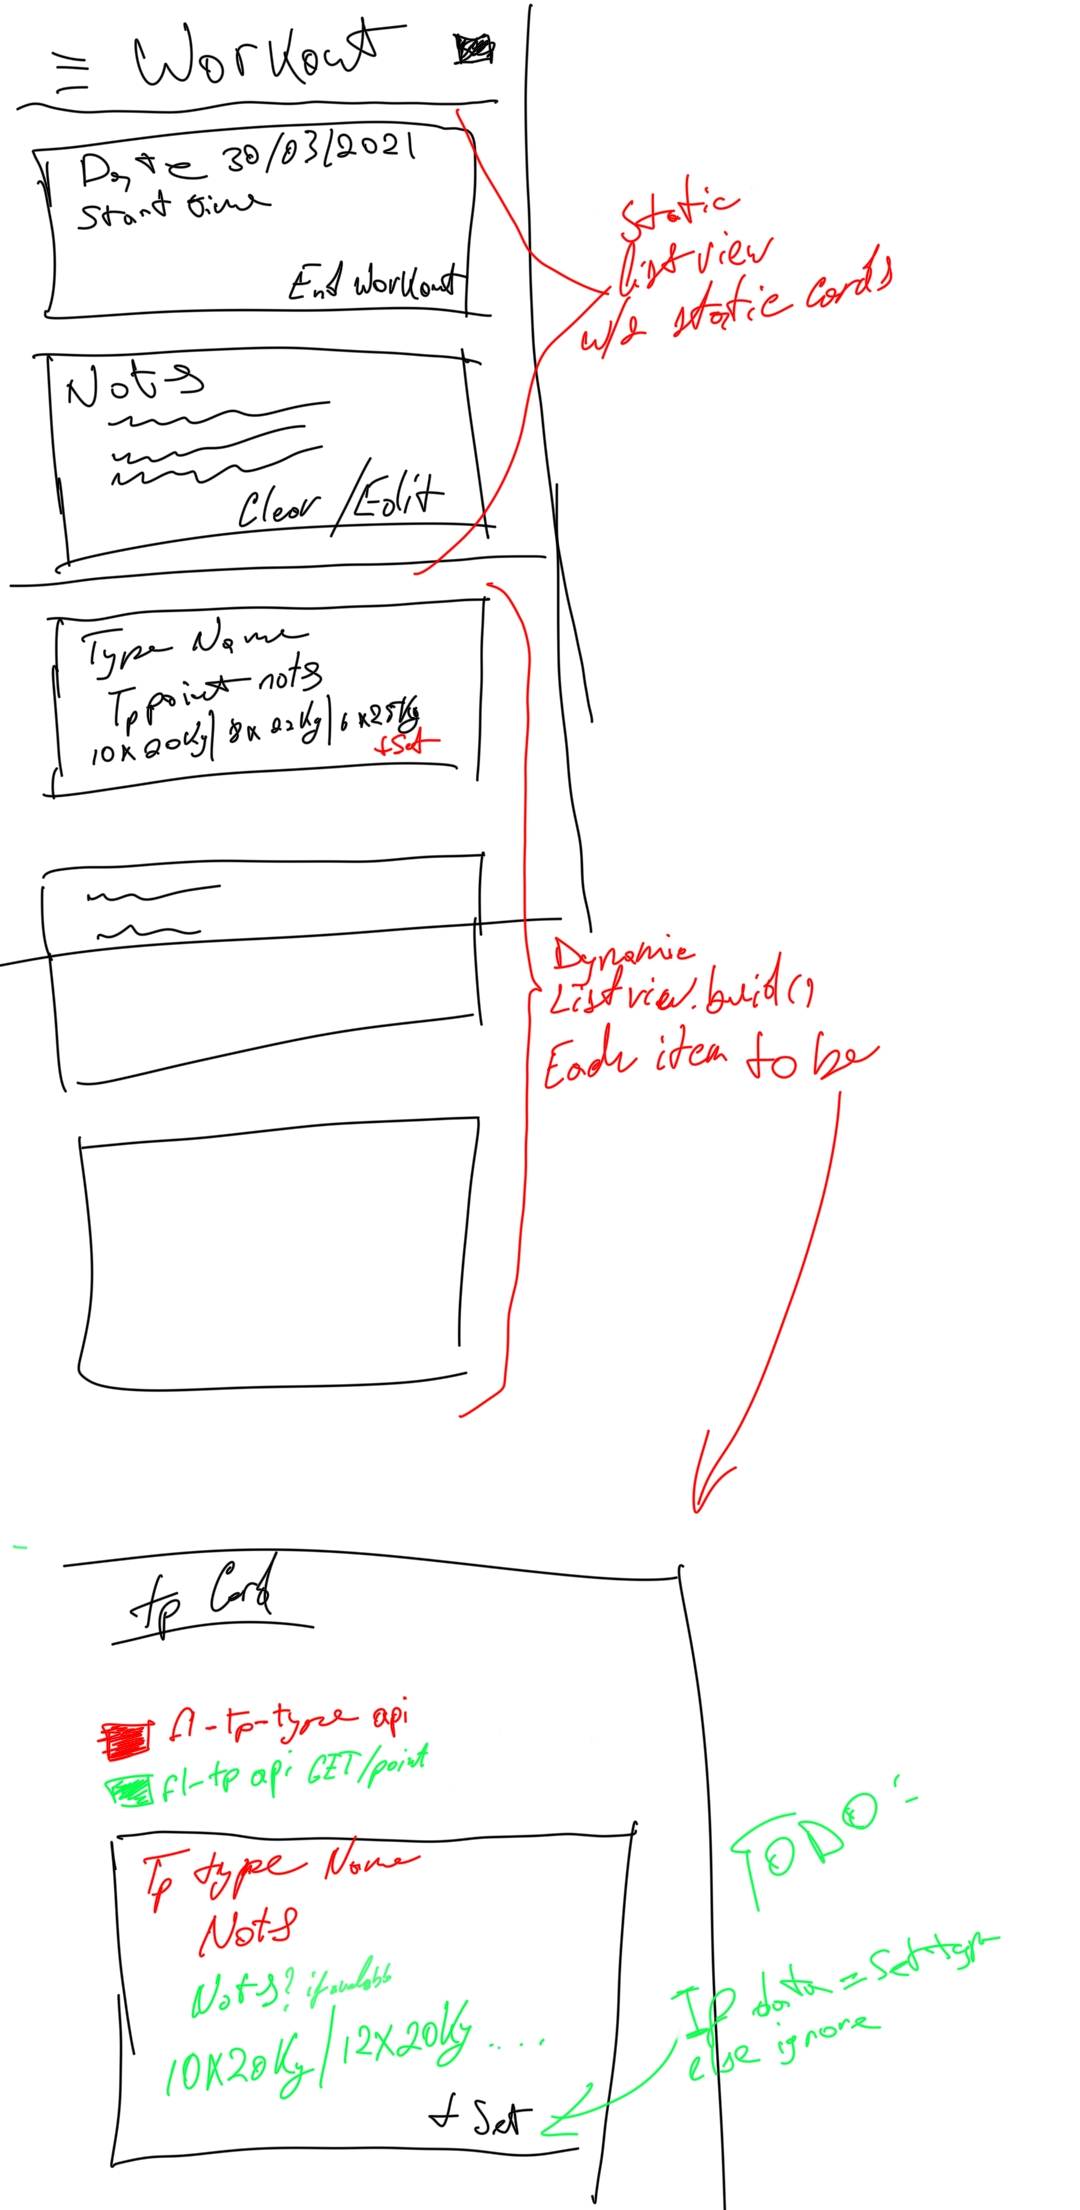
\includegraphics[width=0.9\linewidth]{./appendix/assets/img/uiDesigns/workoutsPage.jpg}
\captionof{figure}{Workout screen design}
~\label{fig:uiWorkoutPageDesign}
\endgroup

\begingroup
\centering
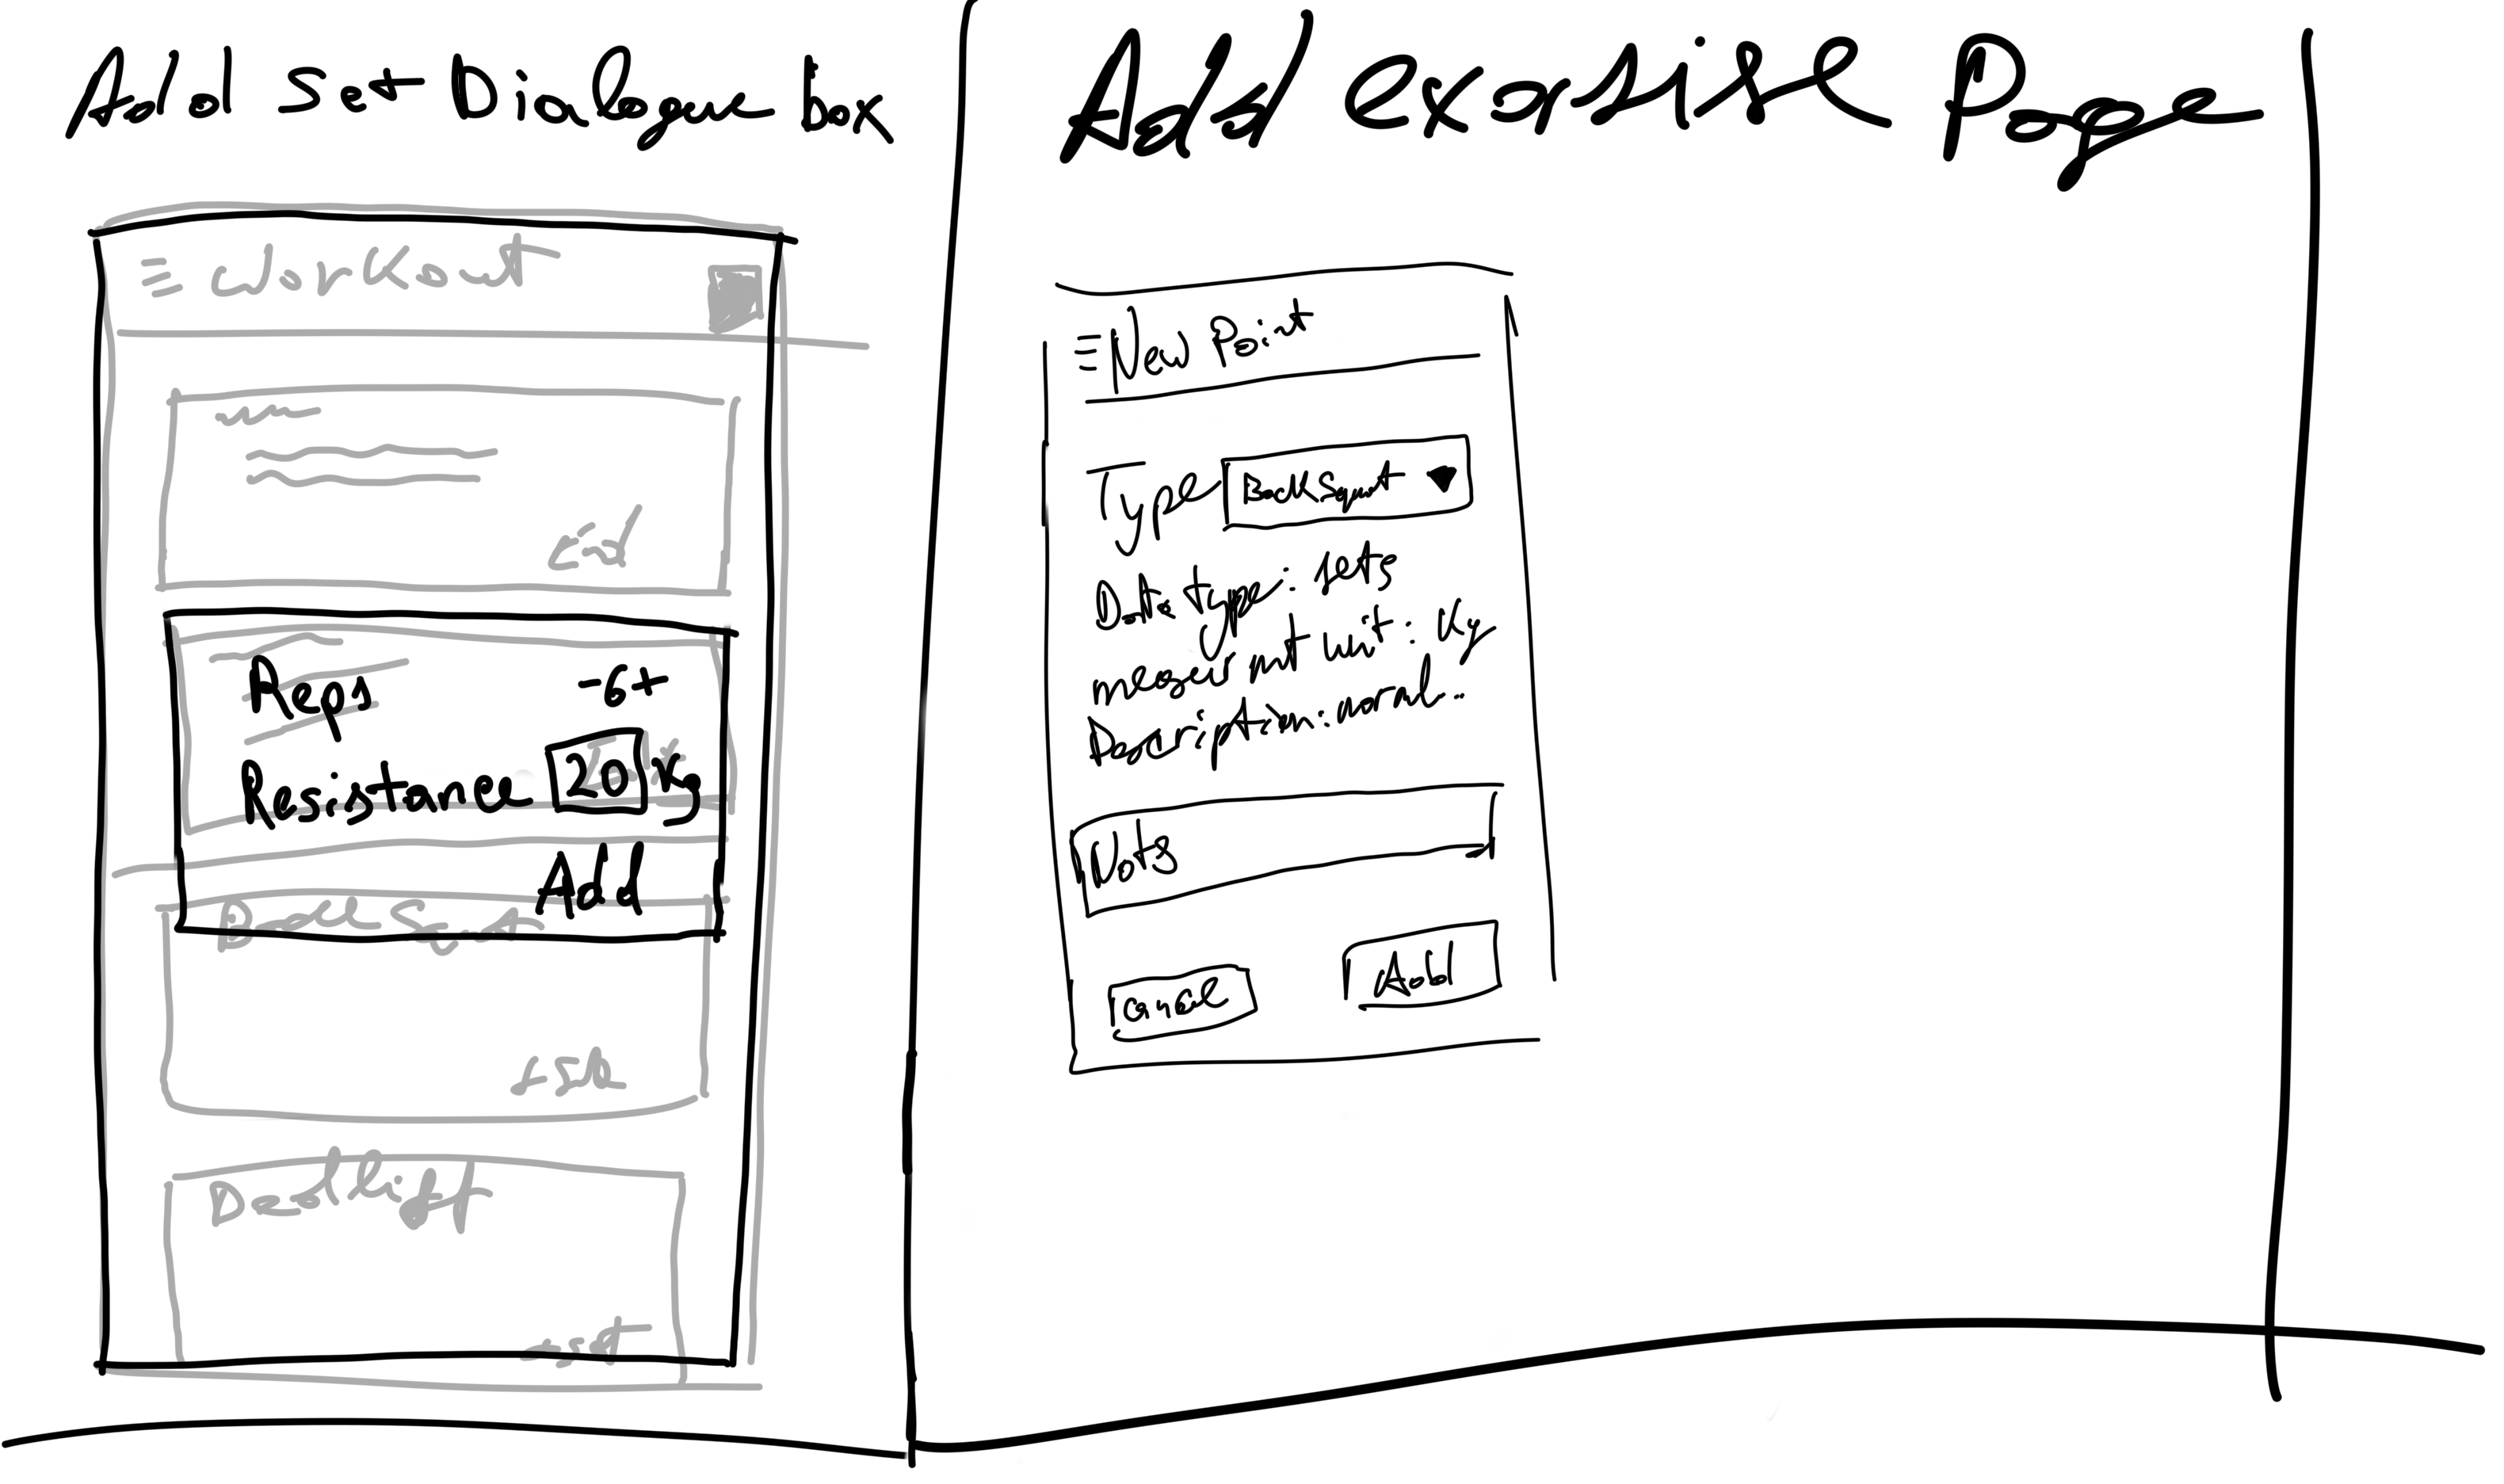
\includegraphics[width=0.9\linewidth]{./appendix/assets/img/uiDesigns/excersisePage.jpg}
\captionof{figure}{Add exercise page and set dialogue.}
~\label{fig:uiExersicePageDesign}
\endgroup

Since the author's main intention with this project was not the UI or overall user experience, this was further down the priority list. However, to aid the UI development, a few sketches were made to help with visualising some specific pages. These page were the workout page, which would display individual \tgs~and their subsequent \tps~(see figure~\ref{fig:uiWorkoutPageDesign}), here the author also specifically modeled each \tp~card and talked about where each piece of data should be coming from. The other sketch in, figure~\ref{fig:uiExersicePageDesign}, shows the design of the add experience page and the add set page.\\

\section{Implementation and Testing}
\vspace{\vspaceconst}

\subsection{Setup}
\vspace{\vspaceconst}
This section will be talking about the different aspects of the setup phase: version control setup, shared code library, template creation and CI/CD.\@

\subsubsection{Version control}
\vspace{\vspaceconst}
The version control management software which has been chosen is Git on GitHub. Other than being simple, Git is also very powerful, specifically in this project, the git-sub module system has been used.  
\begin{quote}
  `Git submodules are simply a reference to another repository at a particular snapshot in time'\cite{atlasianGitSubmodule}
\end{quote}
Originally intended as a dependency tracking system. One project would have a git submodule of some library which exists on another git repository; in a user specified folder, that git repository would be then cloned and a snapshot of it at that current commit. The owner of the parent repository would then be able to use a specified version of the library in their own project as it would be cloned together with the main parent repository.\\
This essentially allows for git repositories to be nested inside one another for better structures. And in this project git submodules was used to separate each individual micro service and the shared code library out into their own repository and CI/CD environment. This separation of repositories is really nice when it comes to working on multiple independent or semi-independent projects that make up a bigger system which would ideally still have one big repository.\\
Consider this use case, each submodule repository has its own CI pipeline where on commits or merges tests and builds are triggered. However, when there is a milestone reached or a version increase, the team could then branch the project parent repository, perform the version bump and then have the CI/CD pipeline of the parent repository perform more builds and tests, here they would even do integration tests with the whole application and not just individually on a per submodule level. So even though all tests and builds pass on the individual submodule, where the team does not need to worry about accidentally triggering builds for the other projects, the new version could have broken something on the bigger project.\\

\subsubsection{Shared code library}
\vspace{\vspaceconst}
Since most of the micro services were written in NodeJS, an NPM\footnote{NPM or Node Package Manager is a package management system that allows one to pull in dependencies from repositories or make their own packages.} was made to share code in-between them. This was necessary because the micro services would be using a lot of the same code like JWT\footnote{JWT or JSON Web Token is an RFC standard for representing security claims\cite{jwtio}.} wrappers, database wrappers, environment variable definitions, data structures and more. Table~\ref{table:flSharedElements} showcases some of the more important elements of the \textit{`fl-shared'} library.\\

\begingroup
\centering
\begin{tabular}{p{2cm} p{5cm}}
  Env wrapper and definition & This has a type definition to tell node which environment variables will exist and provides a wrapper for dealing with env variables.\\
  FlApi & FlApi is a HTTP client which would make calls to neighbouring micro services.\\
  JwtWrapper & This contains helper functions for the JWT lib, but also has express authentication middleware which authorises the users.\\
  Logger & This is a simple std log library, but the idea is that it would be expanded to be able to log on message buses and more.\\
  Models & This is a collection of all the data structures which would be shared across the entire application.\\
\end{tabular}
\captionof{table}{\textit{Fl-shared} elements}
~\label{table:flSharedElements}
\endgroup

\subsubsection{Template for micro services}
\vspace{\vspaceconst}
With micro services it can be very useful to create a bare-bones project with some `hello world' implementation that will define the micro service structure and all of the basic always needed dependencies. This makes is easy to make sure that each project looks structurally similar since they all would start from the same bare-bones project. Additionally this makes the development of new micro services even easier to develop. Such a template was created for this project, simply because during development small changes were made which made sense.

\begingroup
\centering
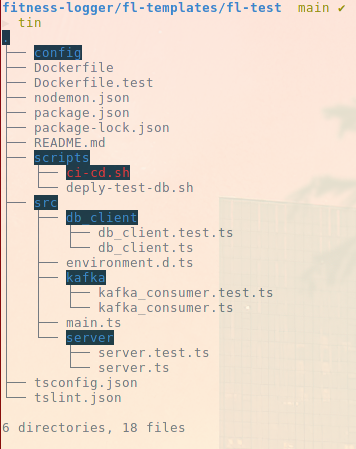
\includegraphics[width=0.5\linewidth]{./appendix/assets/img/flTemplateTree.png}
\captionof{figure}{Fl-template folder structure}
~\label{fig:flTemplateTree}
\endgroup

\begingroup
\centering
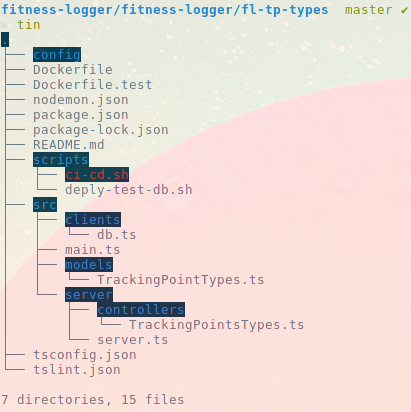
\includegraphics[width=0.5\linewidth]{./appendix/assets/img/flTpTypesTree.png}
\captionof{figure}{Fl-tp-types folder structure}
~\label{fig:flTpTypesTree}
\endgroup

Figure~\ref{fig:flTemplateTree} shows a tree view of the micro service template. As you can see there are some key differences such as a unified clients folder, which would be used for any sort of clients the application would need. However, in addition to that, the kafka client was deleted. In the thought was in the beginning that kafka would be used for asynchronous calls, but in practice, at least for the MVP\footnote{MVP aka minimal viable product.}, there was no need for it so was later removed. Furthermore, the \textit{environment.d.ts} file was removed, the reason for that was the realisation that it was possible to define the environment typings inside the \textit{fl-shared} library.\\

\subsubsection{CI/CD}
\vspace{\vspaceconst}

This is one section which was severely compromised on due to time constraints. On the template micro service, a full CI/CD\footnote{CI/CD or continuous integration and continuous deployment is a pipeline which would be triggered by some event such as a push or a branch merge. The project would then have its unit tests run, the project built and then deployed to a live environment, repository or both.} pipeline was setup, with testing builds and image pushes on the GitHub container registry on every single push to master branch. However, when proper development starter, there simple was not enough time to setup the CI/CD pipeline on every single repository and not enough time to follow test driven development. So in the end, using a script, the container image was built and pushed to the container registry from the main development machine.\\
When it came to the shared NPM module, the pipeline is setup with GitHub actions, just again no actual tests were written, but the test framework has been setup, so this is one of the first items to be on the to-do list for future developments.\\

\subsection{\textit{Fl-auth} service}
\vspace{\vspaceconst}
The \textit{fl-auth} service was the only service to be written in a different programming language, and as mentioned before, it was done so as a proof of concept simply because this was the simplest service to develop. It only has 3 endpoints.\\

\begingroup
\centering
\begin{tabular}{p{2.5cm} p{4.5cm}}
  POST /auth/register & This accepts username, email and password. The password is the hashed with salted and hashed bcrypt\footnote{Bcrypt is a common password hashing function based on the Blowfish cipher.}, then stored in the MongoDB database.\\
  POST /auth/login & This accepts email and password, then it checked the password against the hashed password stored int he database, if a match is made, a JWT token with the appropriate data is generated and sent back.\\
  POST /auth/verify\_me & This accepts the JWT and checks its validity.\\
\end{tabular}
\captionof{table}{\textit{Fl-auth} endpoint}
~\label{table:flAuthEndpoints}
\endgroup

The \textit{`/verify\_me'} endpoint is not actually used. The plan was that it wold be used internally by the other micro services to validate a user's JWT token, however, it was realised that this is not actually needed as with the JWT secret\footnote{JWT secrets are used to generate and to deconstruct the JWT payloads.} it is possible to do that from the other micro services. Although, this endpoint was left in there for possible use by the client, it might even be modified so that it returns the roles which are stored inside it, so that the client is aware of the user's roles. This would be useful in case it is decided to add some form of admin user with admin actions.\\
At the moment authentication service is not actually feature complete. It lacks features such as password recovery proper admin control over the accounts, OAuth\footnote{OAuth\cite{oauth} is an open standard for access delegation, commonly used as a way for Internet users to grant websites or applications access to their information on other websites but without giving them the passwords. This mechanism is used by companies such as Amazon, Google, Facebook, Microsoft and Twitter to permit the users to share information about their accounts with third party applications or websites.} and more. However, it works well enough as a test MVP.\@ In a proper implementation, ideally a system such KeyCloack\cite{keycloack} or Auth0\cite{auth0}.\\
Currently the service generated a JWT based on a JWT claim structure (see code snippet~\ref{code:jwtClaimGo}) which stores all the information about the user, their email, username, user id and an array of roles the user holds.\\

\lstset{language=Golang}
\begin{lstlisting}[escapeinside={(*}{*)}, label={code:jwtClaimGo} ,caption={JWT Claim in Golang}]
type JwtClaim struct {
  ID       string   `json:"id"`
  Username string   `json:"username"`
  Email    string   `json:"email"`
  Roles    []string `json:"roles"`
  jwt.StandardClaims
}
\end{lstlisting}
\lstset{language=TypeScript}

See Section~\ref{section:innerServiceComms} to see how this system has been applied to authenticate communication in-between services.\\

\subsection{\textit{Fl-tp-types} service}~\label{section:flTpTypeImpl}
\vspace{\vspaceconst}

The \textit{fl-tp-types} micro service was the first service to be written in the default stack of NodeJS, typescript and express.  When it comes to the database client, in this service mongoose was used simply because the author was familiar with and the wide support on online forums. However, it can get cumbersome to make both a typescript interface type and a mongoose object defining the document type to manage those separately, so for the next service the author was in search to find another way to use MongoDB.\\
This service is just responsible of dealing with the \tpt~data structure and it just performs crud operations on the database.\\

\begingroup
\centering
\begin{tabular}{p{2.5cm} p{4.5cm}}
  POST /types/ & Add a \tpt\\
  GET /types/ & Get all or search \tpts\\
  PUT /types/ & Modify a \tpt\\
  DELETE /types/ & Delete a \tpt\\
\end{tabular}
\captionof{table}{\textit{Fl-tp-types} endpoint}
~\label{table:flTpTypesEndpoints}
\endgroup

\subsection{\textit{Fl-tp} service}
\vspace{\vspaceconst}
In this service, the usual technical stack was used only with swapping out mongoose for the plain mongo NodeJS driver and using only the builtin typescript interfaces. Validation is just handled in plain logic on the controller side. However, the validation done really is not done on a professional level. Ideally, would build some library component for validation in \textit{fl-shared} or use a library such as \textit{`Joi'} for validation.\\
This service deals with the \tps~the data inside them (sets or single values) and \tgs. Due to the data flow, this service also needs to make calls to \textit{fl-tp-type} (see Section~\ref{section:flTpTypeImpl}).\\
For example, when a new \tp~is created, this service calls the \textit{fl-tp-types} service through a HTTP client wrapper from \textit{fl-shared}. The requests go through the reverse proxy making it easier when the reverse proxy will be migrated to a load balancer.\\

\begingroup
\centering
\begin{tabular}{p{2.5cm} p{4.5cm}}
  GET /tracking/point/ & Get or search a list of all of the \tps~and the data inside them.\\
  POST /tracking/point/ & Add a new \tp.\\
  DELETE /tracking/point/ & Delete a \tp.\\
  POST /tracking/point/set/ & Create a new set at a given \tp.\\
  PUT /tracking/point/set/ & Update a specific set from a given \tp.\\
  GET /tracking/group/ & Get all \tgs.\\
  POST /tracking/group/start & Start a new \tg. Note, one cannot be started of there is one that has not been stopped.\\
  POST /tracking/group/stop & Stop a \tg.\\
  PUT /tracking/group/ & Update a \tp.\\
  DELETE /tracking/group/ & Deletes a specific \tg.\\
\end{tabular}
\captionof{table}{\textit{Fl-tp} endpoint}
~\label{table:flTpEndpoints}
\endgroup

At the moment, this service contains two endpoints, the idea being that \tgs~and \tps~are related to each other. In practice this would have worked just as well as two separate endpoint. So when the `/tracking/point' endpoint needs any \tg~data, it is actually done through the \textit{FlApi} HTTP client from \textit{fl-shared}. This de-couples the two endpoints allowing them to function as two separate entities. This was done to be able to easily separate these two endpoints into different services.\\

\subsection{Inner-service communication}
\vspace{\vspaceconst}
~\label{section:innerServiceComms}

With micro services, inner-service communication is a given requirement. And since it is communicating outside the system the communication needs to be secured and authenticated. In terms of security, that would be done through some encrypted connection such as HTTPs which would be handled on the reverse proxy level of the application.\\
However, authentication is a different topic. It would need to be made sure that micro services would have the necessary permissions for all of the calls performed. Luckily the JWT system made this easy. Since all of the micro services have the JWT secret to de-compile the JWT payload, they can also sign their own JWT tokens. So, in \textit{fl-shared} NPM module, some functions were created to generate a JWT token with a role of `microservice' (see Snippet \ref{code:microServiceJWTGeneration}), this is then injected into every request sent to the reverse proxy and subsequently the requested micro service would check for this role (see Snippet \ref{code:microServiceRoleChecking}).\\

\begin{lstlisting}[escapeinside={(*}{*)}, label={code:microServiceRoleChecking} ,caption={Checking for microservice role.}]
roles[0] === 'microservices' ?
    query.userId = req.query.userId :
    query.userId = res.locals.jwtPayload.id;
\end{lstlisting}

\begin{lstlisting}[escapeinside={(*}{*)}, label={code:microServiceJWTGeneration} ,caption={Generating jwt for microservices.}]
/**
 * Sign the jwt token with env variable.
 *
 * @return string of jwt.
 */
private signJwt(): string {
    const jwtSecret = process.env.JWT_SECRET ?? '';
    const jwtPayload = {
        username: process.env.MS_NAME,
        roles: [MS_ROLE]
    }
    return jwt.sign(jwtPayload, jwtSecret);
}
\end{lstlisting}

When a micro service sees the `microseservice' role, it gets the user id from the URL parameters rather than the JWT payload. This basically lets the micro service perform operations on other endpoint on the behalf of the user.\\

\subsubsection{Dependency injection}
\vspace{\vspaceconst}

Dependency is an often overlooked aspect of application design, on both frontend and backend, and because of that there are many ways of solving the problem, different frameworks like to solve it in different ways. The way dependency injection was done in this application's backend was quite simple. All dependencies are created at the beginning before the HTTP server is started. Usually these would be a database client instance and a HTTP client instance. These would then be passed to the HTTP server's class constructor. From there the client would be injected either on an endpoint basis or server wide (see Snippet~\ref{code:dependencyInjectionWithinServer}) using a middleware\footnote{In this case a middleware is a function which runs before the controller. A middleware can also be used for authenticating requests, if the request is not authentic, then it is sent back with a 401 code before it ever reaches the final controller.} function. Then the injected dependencies would be available from the \textit{`response.locals'} variable on each controller (refer to Snippet~\ref{code:backendDependencyUse}).

\begin{lstlisting}[escapeinside={(*}{*)}, label={code:dependencyInjectionWithinServer} ,caption={Dependency injection within HTTP server.}]
this.app.use((req: Request, res: Response, next: NextFunction) => {
    res.locals.db = this.db;
    res.locals.flApi = this.flApi;
    next();
});
\end{lstlisting}

\begin{lstlisting}[escapeinside={(*}{*)}, label={code:backendDependencyUse} ,caption={Accessing database from locals as an injectable dependency.}]
async function GetTrackingGroups(req: Request, res: Response) {
    const db: DbClient = res.locals.db;
...
\end{lstlisting}

Approaching dependency injection like this is smart because it makes it easy to substitute dependencies, even more so if a template class would be used to implement the dependencies wrapper classes. But also makes it easy to test the application. For unit testing, a mock object class could be injected or even a database setup specifically for testing.\\

\subsection{Android client}
\vspace{\vspaceconst}

For this part of the project, it was decided that Flutter\footnote{Flutter\cite{flutter} is a frontend framework developed by Google, using dart as the core language, it is a framework which compiles to native platforms for building UI applications programmatically.} would be used. Flutter is really good for this use case because it can easily access any of the native components quite easily while being cross platform, compiling for the web, Windows, Linux, MacOS, Android and IOS. This makes it really nice to use because in the future, using the same codebase, the application could be compiled for all the other platforms which would be targeted. The libraries used in this Flutter project were primarily Chopper\cite{chopper} for an easy to use HTTP client and Provider\cite{provider} as a dependency injector.\\
Chopper is nice because one could just create an abstract class, define the API URIs\footnote{A URI is a link localised to a site, in other words the path after the domain in a link.}, data to send and data to receive, then the `build\_runner'\footnote{Flutter package which generates code.} package generated the code for the abstract class. This package makes development a lot nicer, however, there were some difficulties with it. Flutter's latest update, version 2.0, defined a new way to deal with variables which can be null by using a \textit{`?'} operator to define variables which can be null. This means that packages which have not been updated/re-written with compatibility cannot be used in Flutter projects using version 2.0 or higher, and at the time of development Chopper did not have support for that. The right thing would have been to either switch to a different HTTP client library or to use the base HTTP package available in Flutter. However, after some research on the issue, a GitHub milestone\cite{chopperMileStone} and pull requests were found where the maintainers where working on upgrading the package. So it was decided to continue using Chopper, disable null safety\footnote{Null safety is the Flutter 2.0 feature where the Flutter team added support for nullable values} when building the application and to constantly modify the generated code after transpiration in order to make it work with this null safe project as a workaround.\\
The other mentioned package used was Provider. Provider can be used in a lot of different ways, however, in this project it was used as a dependency injection system. At the top of the widget tree\footnote{In Flutter a widget tree is a tree like structure of all of the nested UI classes created. For example a form will have children of text inputs and buttons.} one could use Provider to inject a dependency such as seen in Snippet~\ref{code:flutterProviderInrAuthEx} with the authentication service client example. When it comes to consuming the dependency down the widget tree, its also fairly straight forward. Just one line of code to retrieve it from the current context, see Snippet~\ref{code:flutterProviderOutAuthEx}.\\

\lstset{language=Dart}
\begin{lstlisting}[label={code:flutterProviderInrAuthEx}, caption={Provider injection example with the Authentication service client}]
Provider<AuthService>(
  create: (_) => AuthService(FlAuthApiService.create()),
  dispose: (_, AuthService service) => service.flAuthApiService.client.dispose(),
)
\end{lstlisting}

\begin{lstlisting}[label={code:flutterProviderOutAuthEx}, caption={Provider consuming dependency example with the Authentication service client}]
bool loginAtt = await Provider.of<AuthService>(context, listen: false).login(user)
\end{lstlisting}
\lstset{language=TypeScript}

One quick note on the structure of this application is one missing technical component which would have made the codebase cleaner and easier to develop for would be the inclusion of some state management library such as Bloc\cite{bloc}. Bloc is basically just an event bus for Flutter, it allows for the emission of messages in one place of an application and the listening of those messages in another place.\\

\subsubsection{UI}
\vspace{\vspaceconst}

\begingroup
\centering
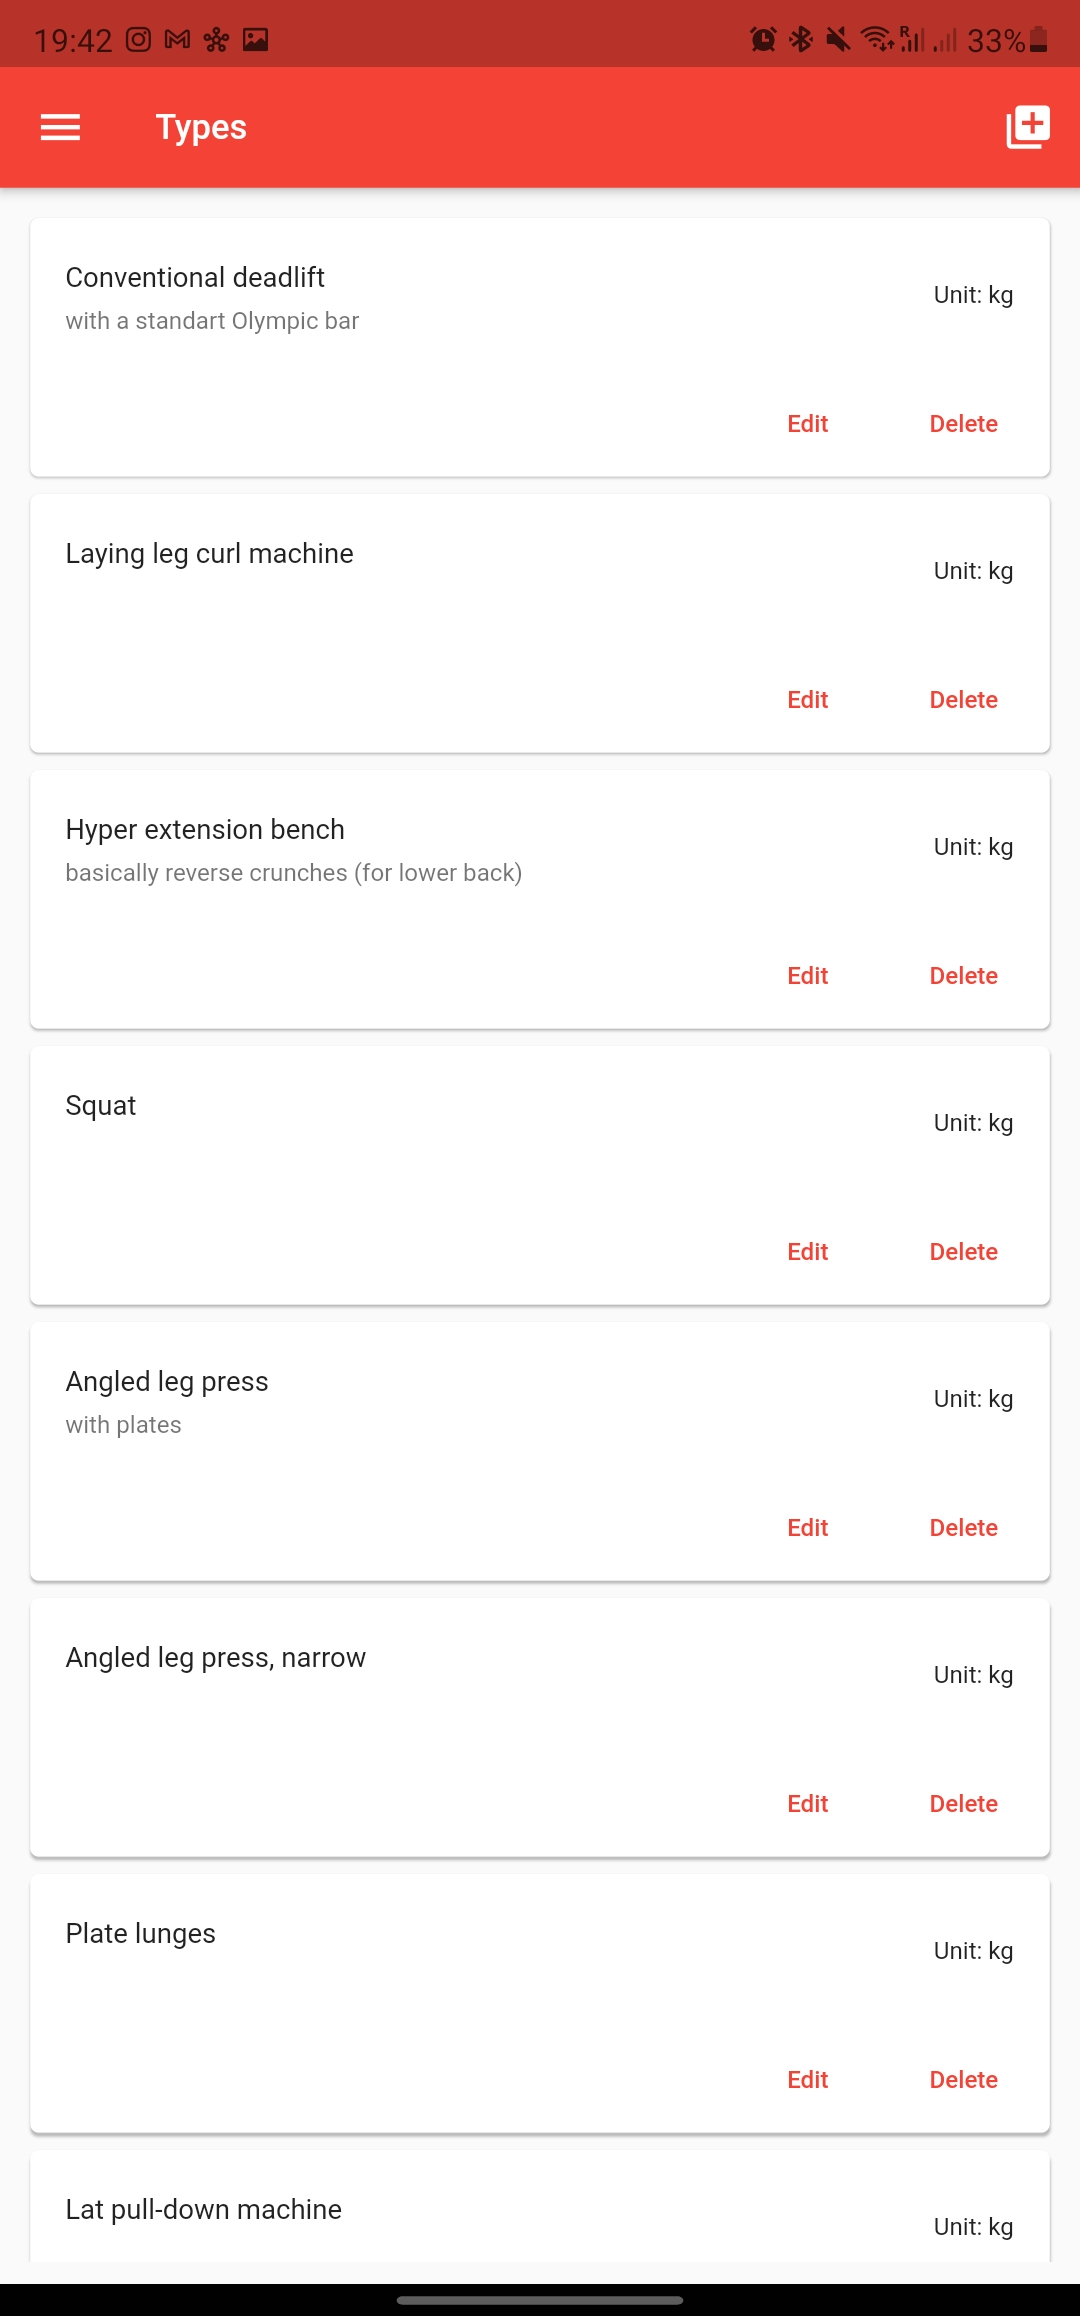
\includegraphics[width=0.7\linewidth]{./appendix/assets/img/uiScreenShots/typesListScreen.jpg}
\captionof{figure}{Custom exercise page screenshot.}
~\label{fig:uiTypesListScreen}
\endgroup

The actual UI of this project was kept relatively simple as there were other more important issues to first tackle during the development of this project. It uses mostly a red and white colour theme and using pre built components from Google's Material UI library\cite{materialUi}. The author tried to keep the design as objectively simple as possible. Here you can see one of the screens, in Figure~\ref{fig:uiTypesListScreen}, which is the custom exercise list page. Here the user will be able to see the list of all the exercises that they have made and is able to create more, edit existent ones or delete them from here using using the add button at the top right of the screen and subsequently the edit or delete button on each listing.

For the features which have not yet been implemented, a toast\footnote{A toast is a small temporary pop-up at the bottom of the screen with information.} with text saying that the feature was not yet implemented. See Figure~\ref{fig:uiToBeImplementedToast} for an example.\\

\begingroup
\centering
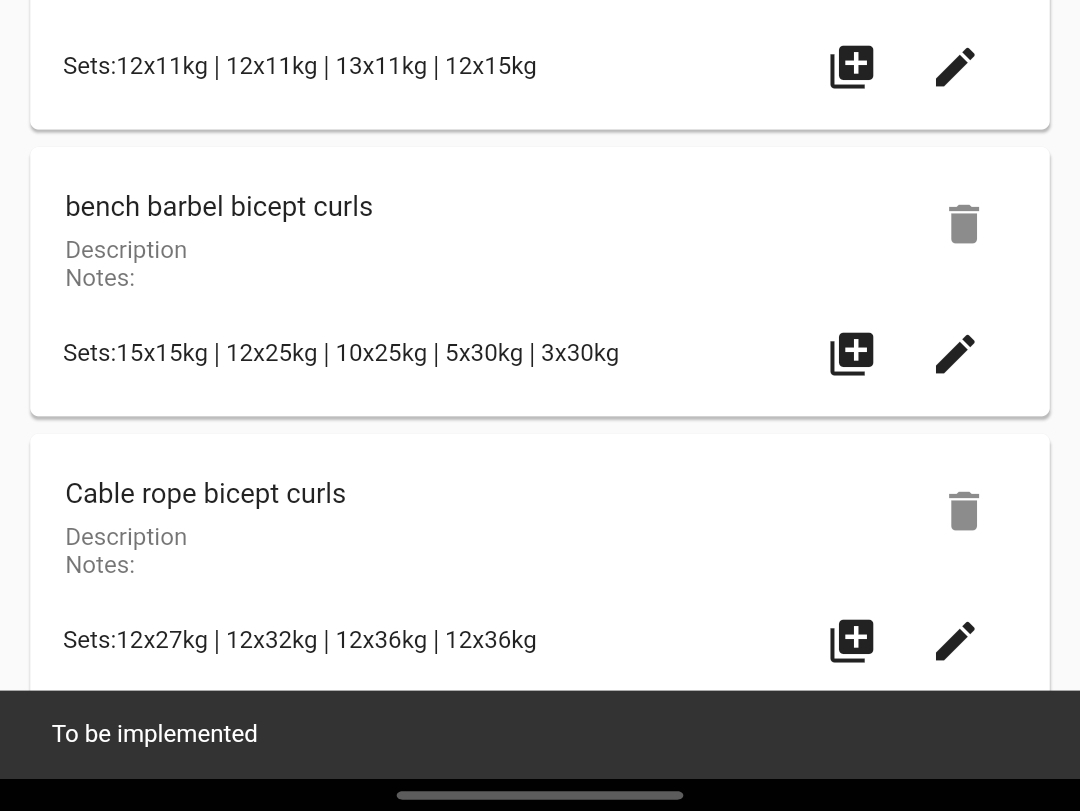
\includegraphics[width=0.7\linewidth]{./appendix/assets/img/uiScreenShots/toBeImplementedToast.jpg}
\captionof{figure}{Toast informing the user that the feature is yet to be implemented.}
~\label{fig:uiToBeImplementedToast}
\endgroup


The following Figure~\ref{fig:uiTypeDeletionDialogue} is one of the confirmation dialogue forms which were used within the application.\\

\begingroup
\centering
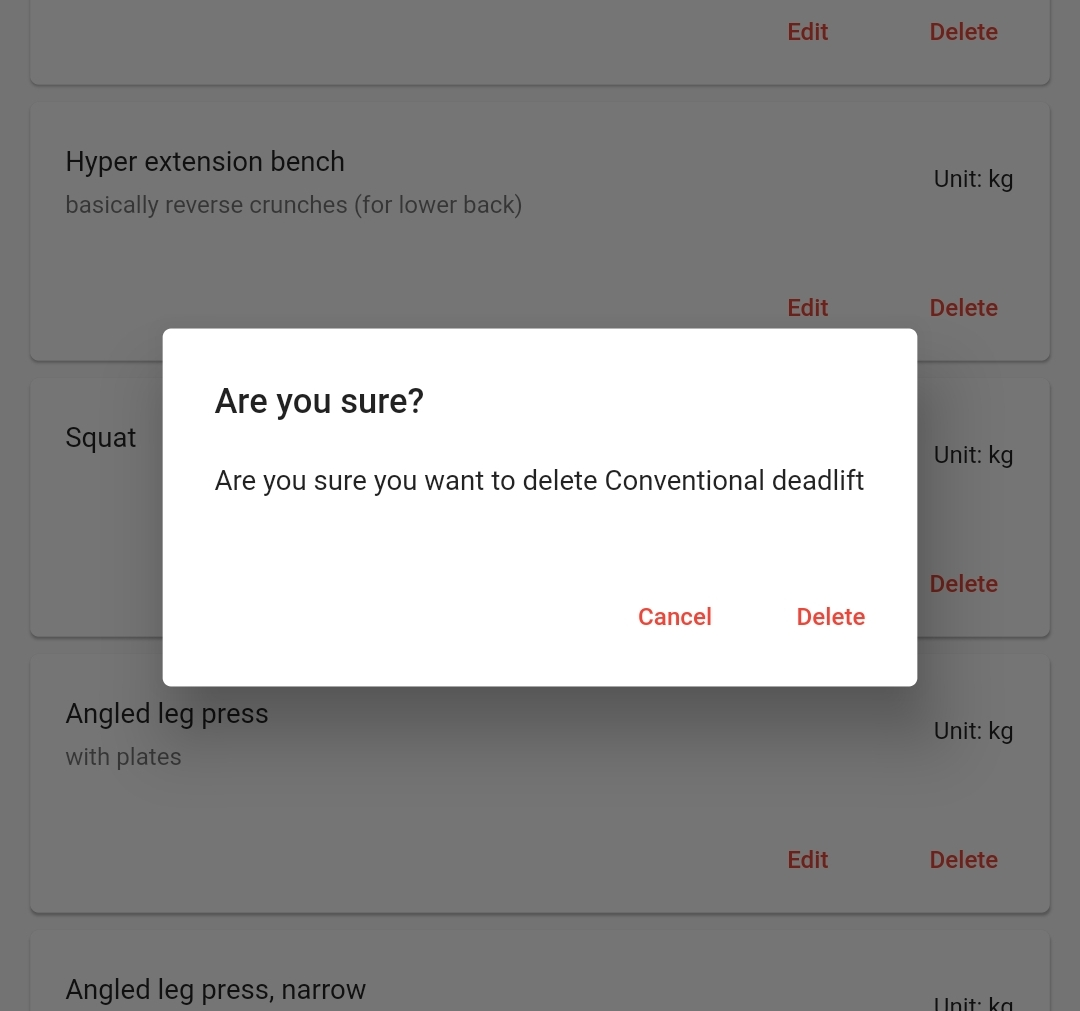
\includegraphics[width=0.7\linewidth]{./appendix/assets/img/uiScreenShots/typeDeletionDialogue.jpg}
\captionof{figure}{Delete custom exercise dialogue.}
~\label{fig:uiTypeDeletionDialogue}
\endgroup

For more examples please refer to the Appendix, in the \textit{`./appendix/assets/img/uiScreenShots/'}.\\

\section{Evaluation}
\vspace{\vspaceconst}

\subsection{Usability}
\vspace{\vspaceconst}

In this project there was not any user testing, reasons being: lack of gym access during the current world situation and the initial focus not being on UI and UX but being on the backend component. And since this project was not centered around the frontend, but around the backend, there was not much need for proper user centered design with UI prototypes. So the only UI designs available are the sketches presented above (see figure~\ref{fig:uiWorkoutPageDesign} and~\ref{fig:uiExersicePageDesign}) which helped with development rather than making the app more usable. However, if development on this app would continue, some user centered design of the UI would definitely be in order. So at this stage, the UI is basically just a way to test the backend, and not much more. Because of this, and partly due to time constraints, it was decided to not perform any user testing.\\
The only testing which was done of the UI was done by the developer himself, which for now was enough because just by using the application as a normal user, the author came up with a few improvements which would be done to the workflow.\\

\subsection{Reflection}
\vspace{\vspaceconst}

The core concept of this project was achieved. The application used micro services backed application, which in theory would allow for easier scalability in the future, offers better code encapsulation\footnote{Code encapsulation in the sense of splitting up different parts of the application.} of backend functions, making development easier with new future releases, and making it easier for multiple teams to collaborate if there is a future need for it. And the other part of the project being simplifying the workout logging such that it could be used simply in a multitude of ways.\\
The one part of the project which had to be left out was the \textit{`fl-analytics'} micro service or any other analytical part of the client. Due to time constraints this had to be left out of the MVP and be changed to a stretch goal which was never reached in the end.\\

\subsubsection{Code Quality}~\label{section:codeQuality}
\vspace{\vspaceconst}

Because of time constraints, there needed to be some corners cut during the development of this project, so, the quality of the work could also be improved by a lot. Beginning with the fact that the whole project needs to be covered in unit tests and mocks for different tests. For example the database could be mocked or it just be a test database, but the different services would definitely need to be mocked for other services when testing. With that said, the \textit{`fl-shared'} library would also need to have unit tests implemented.\\
One other obvious place where the code is of poor quality is the user validation on the API side. This is really important because at the moment there is nothing stopping the user from making their own API calls outside the application, so there could be security implications, simply data integrity implications and even server brashest. Although, because the application is deployed with \textit{`docker-compose'}, it was specified in the configuration to restart the containers whenever the crash.\\
The frontend especially if of quite poor quality too. It does not have a standardised library of components, it does not have any proper state management system, it does not have any unit tests and there are a fair amount of bugs which would need to be researched and fixed. For example, in the workout screen (see Figure~\ref{fig:uiTypesListScreen}) there exists a bug which does not update the custom exercise properly, and it might not even update the right record, as just mentioned, it needs some research and troubleshooting.\\

\subsection{Future plans}
\vspace{\vspaceconst}

First and foremost, the whole application would need to be covered in unit tests and possibly some integration test. This will allow the author, or a possible development team to be able to maintain, edit and create new features without having worrying about introducing bugs in another part of the application. One of the tricky problems with this is on the backend. Because there are some micro services which depend on others, some mocking~\footnote{Mocking is when, in a unit test, the developer would create functions or classes returning mock data, replacing the different dependencies that the unit test might need.} will need to be done. A good way of doing that would be to have mock classes in a shared NPM module, this would allow for easy maintenance and modification whenever the actual service is being updated, also for the sake of not having to individually mock each service when one service is dependant on another.\\
On the frontend it is likely that a whole re-write would have to be done. First of all, there would need to be proper designs done in something like AdobeXD\cite{adobexd}, of both individual components (like buttons and input boxes) and of whole screens. This design would of course need to be user centered. Then, the component library would need to be built, simply so it could be used across the entire application. All of this would need to be unit tested too. When building developing the actual client app, a state management like Bloc will be used. This is simply so that the application can properly keep track of the state of different components and give them the ability to change states. This should help with bugs such that were mentioned in Section~\ref{section:codeQuality} where the information on the screen was not updating properly after an update. One last problem which would need to be fixed from the old codebase is the HTTP client, there will need to be a spike\footnote{Spike, a term from agile development, is when you have a story task to just complete research on a topic, usually with a cutoff date.} to determine if the Chopper library used before is appropriate to use or if it needs to be swapped out for something else. The author's current thoughts are that the base HTTP library is simple enough to use and might just need a custom simple wrapper around it before creating the service clients.\\
When it comes to taking the application to market, there would need to be more market research to done. First thing would be to talk to some personal trainers and coaches, to get their opinion on what different types of logs could look like. Next, there would be a survey or an in person interview with a selection of athletes, to see what their workout loggers look like.\\
Next up would be coming up with a way to monetise the application. One popular option is to have a free version with advertisements and less features, and a paid one without advertisements and with all the features enabled. However, another better option would be to have the free one be an offline only application with some features not working because there would be a need of connectivity to the servers. Then a paid one (paid in regular intervals as to be able to keep the servers running) with all the features working. This approach would mean that only paid customers are putting load on the backend infrastructure and the free application serves as a demo without putting a load on the servers.\\
One last item which would need to be implemented is cashing\footnote{Cashing is when information is kept in memory and reused, this is done in order to reduce the amount of calls to a resource are made or to improve speed, since RAM is faster than all other I/O operations.}, on both the server side and the client side. On the server side there is not actually much which could be cashed, however that could change in the future with addition of extra features. However performing cashing on the on the client side would reduce the number of calls by a great amount making the system more efficient.\\


\subsubsection{Features}
\vspace{\vspaceconst}

Once all of the code refactoring, unit test coverage, necessary designs and market research is done, new features will start to be added to the project, some from the stretch goals that the project had and some new ones which the author thought about during development but which were never included in the project because they were out of scope for the current iteration.\\
Firstly, a micro service for compiling reports and other analytical information is getting created. That micro service will get triggered by an event system like Kafka, it will then get information from the different micro services, calculate different statistics about them and make it available to the user. For example, the user would be able to see progress over time on certain exercises or workouts, and on completion of each workout they would have a report of the workout ready to download. This feature would get pulled in from the stretch goals.\\
Another feature which would make this project sand out amongst other similar applications would be a tagging system. This tagging system would have the ability to create custom tags and apply them to anything in the system, custom types, workouts, \tps, etc. Then when generating analytical data, they would be used to compile custom reports and charts. For example a user could create a tag of \textit{`#badsleep'} and the user could apply this tag to any workout where they had bad sleep. Then when creating reports or custom graphs, they can make the analytical system not include the workouts where the user had bad sleep. Another way in which this tag system could be used would be to make tags for the different muscles to be used in an exercise or workout.\\
A longer term feature which the author wants to research is a system for using the phones camera to check the form of the user's exercise\footnote{The form of an exercise is the way in which the athlete performs said exercise, it is important to have good form because could be cause from improper training.}. This would be using computer vision and machine learning in order to detect the form and give feedback. This would be a very powerful feature considering that at the moment there are only really two ways of learning the correct form of exercises. Getting a coach/personal trainer, which is the best option out of the two, however, it can be quite costly. Or, the athlete teaching the proper form himself, out of books, web sites and videos. The latter option is not the greatest because a person could teach themselves the wrong form, which could cause injuries in the long terms, but also will make it harder to learn the proper form in the future.

\section{Description of the Final Product}
\vspace{\vspaceconst}

Just like many other projects, the current version of this one is made up of primarily two components, a backend and a frontend. However, as it was mentioned before, this project was developed with a focus on the backend architecture first and everting else second. 

\subsection{Backend Services}
\vspace{\vspaceconst}

The backend is mainly split into a few different parts, the three micro services which were developed, the shared code library for those micro services, the reverse proxy which routs traffic to the services and the database. At this end of this section, there will also be an outline of how everything was deployed.

\subsubsection{Fl-Auth Service}
\vspace{\vspaceconst}

The authentication service is probably the simplest service. It has the ability to register new users and to log in the new users. At this point in time features such as password recovery and OAuth have not been implemented.

\subsubsection{Fl-Tp-Types Service}
\vspace{\vspaceconst}

The types service is responsible of the storage of different \tpts~the user will create (all of the basic CRUD operations). Usually they will be exercises, however, they can be used for just about anything the users wants. For example, one the author at the moment has two non-exercise \tpts~, one for tracking caffeine intake before a workout, and another for logging amount of calories burnt during a workout (this information is manually tracked by a fitness band).\\
It was mentioned before that there is a bug with updating \tpts~, it is likely that the problem is here in the \textit{`PUT'} controller of this service.\\

\subsubsection{Fl-Tp Service}
\vspace{\vspaceconst}

The tracking point service is the service which deals with \tgs~(or workouts) and with \tps~(or exercise logs). This is the service which gets used whenever there the user is logging an actual workout. In this version of the project, this is the only service making any calls to other services.\\

\subsubsection{Fl-Shared NPM module}
\vspace{\vspaceconst}

The shared NPM module is used for any code which could be re-used for any other service, it contains code such as HTTP client wrappers, type declarations, miscellaneous functions, authentication middleware and more.\\

\subsubsection{Fl-proxy Service Proxy}
\vspace{\vspaceconst}

The service proxy at the moment has two basic jobs. One is two cover the entire backend with a HTTPS certificate, and the second is to forward traffic to all of the different service. This way there is only one endpoint open to the internet under port 80 or 443. If each individual service were to be open to the internet, they would need to be open under different ports, which can become messy. For instance, the \textit{fl-tp-types} service is forwarded all of the traffic from \textit{`/types'} URI.\\

\subsubsection{Database}
\vspace{\vspaceconst}

\subsubsection{Deployment}
\vspace{\vspaceconst}

A VPS\footnote{VPS meaning virtual private server.} was used for deploying the backend services, in specific one from Digital Ocean\cite{digitalOcean}. The server is running Docker and is configured with docker-compose. Two main docker-compose configuration files were made, one for the micro services and the proxy, another for services such as the database. This was done to simply avoid unnecessary restarts of the database or any message bus service which could be used.\\
\\
\subsection{User Interface}
\vspace{\vspaceconst}

As it was mentioned above, the user interface, or client, is an Android application which was made for the purpose of consuming the backend API endpoints.\\

\subsubsection{Login Screen}
\vspace{\vspaceconst}

In appendix 5.(d) you can see the login screen created for the application. On this version of the application this just allows the user to login using their credentials. Due to time constraints and beta purposes, the registration feature has not been implemented.\\

\subsubsection{Home Screen}
\vspace{\vspaceconst}

In appendix 5.(i) you can see the home screen. This is basically just a menu to launch the types list page and the workouts list page.\\

\subsubsection{Types}
\vspace{\vspaceconst}

In appendix 5.(n) you can see the types list screen. This is where all custom user types will be displayed. Mentioned above was a bug which this screen had. The bug occurs when editing a type. The author has not yet found the exact cause nor documented the exact behaviour of the bug as it is not constant.\\
Furthermore, in appendices 5.(j) and 5.(m) you can see the same page which is the same screen, however, reused for editing a type (by pre-populating the fields with the existing information) or for creating a new type.\\
Appendix 5.(o) is a dialogue box which gets a confirmation from the user if they want to delete the type.\\

\subsubsection{Workouts}
\vspace{\vspaceconst}

In appendix 5.(p) you can see a list of workouts that the user has had in the past. If a workout is ongoing the user will also see that one. Here the workouts are listed in reverse order with the newest one on the top. On this screen the user can start another workout with the button on the top right corner, view a specific workout or delete one.\\
Following up is appendix 5.(g), here you can see the screen which displayed the information about one specific workout. If the workout is ongoing, there will be buttons to end the workout, a stop button at the top right and an end workout text button on the bottom right of the first card. Bellow the line which comes after the second card, there is a list of all exercises or \tps~which have been logged for that specific workout.\\
When stopping a workout, there is also a dialogue box confirming that action(see appendix 2.(e)).\\
Each \tp~card shows information about the \tp~and about its respective \tpt. On each card there are three buttons if the \tpt~is using sets and two buttons if its using single values. The two buttons which are always there are an edit pencil icon button and a delete icon button, both of these do not work at this moment and just trigger a notification toast explaining that the feature has not been implemented (see appendix 5.(h)). The other button which appears on set types opens a new set dialogue box (see appendix 5.(q)).\\
When adding a new exercise, or \tp~(see appendix 5.(l)) you can can chose from different types with a drop down (see appendix 5.(c)), or, from here you can also access the add new types screen with the add new type button. Once selecting a type, the information for that type will be displayed. In case the type is of a single value type, it will also display an input box for that single value (see appendix 5.(b)). Appendix 5.(a) is just with the set type.\\


\subsubsection{Hamburger Menu}
\vspace{\vspaceconst}

The hamburger menu is quite simple, see appendix 5.(r). It only has two buttons, one for the home screen and another to logout and send the user to the login page.\\


\section{Conclusion}
\vspace{\vspaceconst}

To conclude, the two main problems which the author was attempting to solve was the problem of logging fitness workouts and the general problems of application development which can be solved with using a micro services approach. In the author's opinion, the solution to both problems have been successful to varying degrees. One find when it comes to micro services was that sometimes it will be introducing just too much complexity, and when talking about this project specifically, the same can be said. The facts of the matter is that this specific project is too small to gain any real benefits from using this approach. However, the author has achieved his goal of learning this architecture and will be confident in the future when applying this knowledge for other projects.\\
When talking about the fitness logging problem, in the author's personal opinion this was a successful proof of concept, the solution still needs a lot of work, especially on the frontend side, however, the system is functional and flexible enough to be used with complex workouts.\\
The main problem which are left are just problems of user experience and general usability of the actual application. However, that can be all solved given more time.\\

\section*{Acknowledgements}
\vspace{\vspaceconst}
First and foremost I would like the to thank my advisor, Andrew Colby for guiding me through this project. One other person which deserves a mentions is my colleague Andrius Navasaitis for helping along while I was getting myself familiar with micro services. Last but not least a big thanks goes to my family, friends and god for all of the support during these uncertain, and mentally draining times\cite{uncertainTimes} we all live in.\\

\newpage
\section*{Appendices}
\vspace{\vspaceconst}

All of the links bellow are relative to the appendix folder which is located at this GitHub url: \url{https://github.com/JamesTiberiusKirk/fitness-logger/tree/master/docs/final-report/tex/appendix/}. Please note that the author's GitHub username is JamesTiberiusKirk.
\begin{enumerate}
  \item Charts:
    \begin{enumerate}
      \item Project overview in draw.io format: \textbf{assets/charts/fitnessLogger.drawio}\\  
      \item Project overview in PNG format: \textbf{assets/charts/fitnessLogger.png}\\  
      \item Project overview in JPEG format: \textbf{assets/charts/fitnessLogger.jpg}\\
    \end{enumerate}
  \item Miscellanies Images:\\
    \begin{enumerate}
      \item Backend backlog and Kanban: \textbf{assets/img/backendBacklog.jpg}\\
      \item Micro service template folder structure: \textbf{assets/img/flTemplateTree.png}\\
      \item Frontend backlog and Kanban: \textbf{assets/img/frontendBacklog.jpg}\\
      \item Initial Requirement Document: \textbf{assets/img/initialRequirementDocument.jpg}\\
      \item Folder structure of fl-tp-types service: \textbf{assets/img/flTpTypesTree.png}\\
    \end{enumerate}
  \item Example journal entries:
    \begin{enumerate}
      \item \textbf{assets/img/journalEntries/ex1.jpg}\\
      \item \textbf{assets/img/journalEntries/ex3.jpg}\\
      \item \textbf{assets/img/journalEntries/ex2.jpg}\\ 
      \item \textbf{assets/img/journalEntries/ex4.jpg}\\ 
    \end{enumerate}
  \item UI Designs:
    \begin{enumerate}
      \item Exercise page: \textbf{assets/img/uiDesigns/excersisePage.jpg}\\
      \item Workouts page: \textbf{assets/img/uiDesigns/workoutsPage.jpg}\\ 
    \end{enumerate}
  \item Finished UI screenshots:
    \begin{enumerate} 
      \item Tracking points new set screenshot: \textbf{assets/img/uiScreenShots/trackingPointNewSet.jpg}\\
      \item Tracking point new single value screenshot: \textbf{assets/img/uiScreenShots/trackingPointNewSingleValue.jpg}\\
      \item Tracking point new type list screenshot: \textbf{assets/img/uiScreenShots/trackingPointNewTypeList.jpg}\\
      \item Login page screenshot: \textbf{assets/img/uiScreenShots/loginScreen.jpg}\\ 
      \item Workout stop dialogue screenshot: \textbf{assets/img/uiScreenShots/workoutStopDialogue.jpg}\\
      \item Workout edit notes Dialogue: \textbf{assets/img/uiScreenShots/workoutEditNotesDialogue.jpg}\\ 
      \item Workout screen screenshot: \textbf{assets/img/uiScreenShots/workoutScreen.jpg}\\
      \item To be implemented toast screenshot: \textbf{assets/img/uiScreenShots/toBeImplementedToast.jpg}\\
      \item Home screen screenshot: \textbf{assets/img/uiScreenShots/homeScreen.jpg}\\ 
      \item Type edit screen screenshot: \textbf{assets/img/uiScreenShots/typeEditScreen.jpg}\\
      \item New workout screen screenshot: \textbf{assets/img/uiScreenShots/newWorkout.jpg}\\
      \item New tracking point screen screenshot: \textbf{assets/img/uiScreenShots/trackingPointNew.jpg}\\
      \item New types screen screenshot: \textbf{assets/img/uiScreenShots/typeNewScreen.jpg}\\
      \item Types list screen screenshot: \textbf{assets/img/uiScreenShots/typesListScreen.jpg}\\
      \item Type deletion dialogue screenshot: \textbf{assets/img/uiScreenShots/typeDeletionDialogue.jpg}\\
      \item Workouts list screen screenshot: \textbf{assets/img/uiScreenShots/workoutsListScreen.jpg}\\
      \item Set add dialogue screenshot: \textbf{assets/img/uiScreenShots/setAddDialogue.jpg}\\
      \item Hamburger menu screenshot: \textbf{assets/img/uiScreenShots/hamburgerMenu.jpg}\\
    \end{enumerate}
  \item Advisor meeting notes and minutes:
    \begin{enumerate}
      \item \textbf{assets/img/advisorMeetingNotes/ex1.jpg}\\
      \item \textbf{assets/img/advisorMeetingNotes/ex3.jpg}\\
      \item \textbf{assets/img/advisorMeetingNotes/ex2.jpg}\\
    \end{enumerate}
  \item User documentation and demo video on youtube: \url{https://youtu.be/qksEcqVqvK4}\\
  \item Fitness logger android app APK 0.0.1 release: \url{https://github.com/JamesTiberiusKirk/fitness\_logger\_app/releases/tag/0.0.1}\\
    \begin{enumerate}
      \item Demo account details are as follows:\\
      \item email: `test@gmail.com'\\
      \item password:`testPass'\\
      \item For any difficulties or a different/private account please contact the author.
    \end{enumerate}
  \item Fitness Logger full source code: \url{https://github.com/JamesTiberiusKirk/fitness-logger/}
\end{enumerate}

\newpage
\begin{thebibliography}{9}

  \bibitem{Docker}
  Docker website (April 2021).\\
  \url{https://www.docker.com/}

  \bibitem{k8s}
  Kubernetes website (April 2021).\\
  \url{https://kubernetes.io/}

  \bibitem{grpc}
  gRPC website (April 2021).\\
  \url{https://www.grpc.io/}

  \bibitem{kafka}
  Kafka website (April 2021).\\
  \url{https://kafka.apache.org/}

  \bibitem{linkerd}
  Linkerd website (April 2021).\\
  \url{https://linkerd.io/}

  \bibitem{istio}
  Istio website (April 2021).\\
  \url{https://istio.io/}
  
  \bibitem{atlasianGitSubmodule}
  Git sub module documentation from Atlasian (April 2021).\\
  \url{https://www.atlassian.com/git/tutorials/git-submodule}
 
  \bibitem{jwtio}
  JWT.io website (April 2021).\\
  \url{https://www.jwt.io}

  \bibitem{auth0}
  Auth0 website (April 2021).\\
  \url{https://auth0.com/#!}

  \bibitem{keycloack}
  KeyCloack website (April 2021).\\
  \url{https://www.keycloak.org/}

  \bibitem{oauth}
  Oauth 2.0 RFC documentation (April 2021).\\
  \url{https://tools.ietf.org/html/rfc6749}

  \bibitem{flutter}
  Flutter website (April 2021)
  \url{https://flutter.dev/}

  \bibitem{chopper}
  Chopper repository (April 2021).\\
  \url{https://pub.dev/packages/chopper}

  \bibitem{chopperMileStone}
  Chopper github repository milestone (April 2021).\\
  \url{https://github.com/lejard-h/chopper/milestone/2}

  \bibitem{provider}
  Provider repository (April 2021).\\
  \url{https://pub.dev/packages/provider}

  \bibitem{bloc}
  Bloc repository (April 2021).\\
  \url{https://pub.dev/packages/flutter\_bloc}

  \bibitem{zerotohero}
  Zero to hero play store listing (April 2021).\\
  \url{https://play.google.com/store/apps/details?id=com.mappz.zerotohero&hl=en\_US&gl=US}

  \bibitem{agile}
  Agile elevator pitch from Atlasian (April 2021).\\
  \url{https://www.atlassian.com/agile}

  \bibitem{materialUi}
  Google's material UI website (April 2021).\\
  \url{https://material-ui.com/}
  
  \bibitem{adobexd}
  Adobe website (April 2021).\\
  \url{https://www.adobe.com/products/xd.html}

  \bibitem{digitalOcean}
  Digital Ocean website (April 2021).\\
  \url{https://digitalocean.com}

  \bibitem{uncertainTimes}
  Information on these uncertainm times (April 2021).\\
  \url{https://www.nhs.uk/conditions/coronavirus-covid-19/}
\end{thebibliography}
\newpage
\end{multicols}
\end{document}
